\PassOptionsToPackage{svgnames}{xcolor}
\documentclass[12pt]{article}



\usepackage[margin=1in]{geometry}
\usepackage{graphicx}
\usepackage{amsmath}
\usepackage{amsfonts}
\usepackage{amsthm}
\usepackage{amssymb}
\usepackage{array}
\usepackage{thmtools} 
\usepackage{bm}
\usepackage{pdfpages}
\usepackage{mathtools}
\usepackage{tabularx}
\DeclareFixedFont{\ttb}{T1}{txtt}{bx}{n}{12} % for bold
\DeclareFixedFont{\ttm}{T1}{txtt}{m}{n}{12}  % for normal

% Custom colors
\usepackage{color}
\definecolor{deepblue}{rgb}{0,0,0.5}
\definecolor{deepred}{rgb}{0.6,0,0}
\definecolor{deepgreen}{rgb}{0,0.5,0}

\usepackage{listings}

% Python style for highlighting
\newcommand\pythonstyle{\lstset{
language=Python,
basicstyle=\ttm,
otherkeywords={self},             % Add keywords here
keywordstyle=\ttb\color{deepblue},
emph={MyClass,__init__},          % Custom highlighting
emphstyle=\ttb\color{deepred},    % Custom highlighting style
stringstyle=\color{deepgreen},
frame=tb,                         % Any extra options here
showstringspaces=false            % 
}}


% Python environment
\lstnewenvironment{python}[1][]
{
\pythonstyle
\lstset{#1}
}
{}
\newcolumntype{Y}{>{\centering\arraybackslash}X}
% Python for external files
\newcommand\pythonexternal[2][]{{
\pythonstyle
\lstinputlisting[#1]{#2}}}

% Python for inline
\newcommand\pythoninline[1]{{\pythonstyle\lstinline!#1!}}
\DeclarePairedDelimiter\ceil{\lceil}{\rceil}
\DeclarePairedDelimiter\floor{\lfloor}{\rfloor}
\newcommand{\sectionline}{%
  \noindent
  \begin{center}
  {\color{DarkViolet}
    \resizebox{0.5\linewidth}{1ex}
    {{%
    {\begin{tikzpicture}
    \node  (C) at (0,0) {};
    \node (D) at (9,0) {};
    \path (C) to [ornament=85] (D);
    \end{tikzpicture}}}}}%
    \end{center}
  }
 \newcount\colveccount
\newcommand*\colvec[1]{
        \global\colveccount#1
        \begin{pmatrix}
        \colvecnext
}
\def\colvecnext#1{
        #1
        \global\advance\colveccount-1
        \ifnum\colveccount>0
                \\
                \expandafter\colvecnext
        \else
                \end{pmatrix}
        \fi
}
 \newcommand{\im}{\mathrm{i}}
  \newcommand{\diff}{\mathrm{d}}
\setlength{\parindent}{0cm}
\setlength{\parskip}{0em}
\let\definition\relax
\let\theorem\relax
\let\corollary\relax
\let\lemma\relax
\let\proposition\relax
\let\algorithm\relax
\declaretheorem[name=Definition,numbered=no]{definition}
\declaretheorem[name=Theorem,numbered=no]{theorem}
\declaretheorem[name=Corollary,numbered=no]{corollary}
\declaretheorem[name=Lemma,numbered=no]{lemma}
\declaretheorem[name=Proposition,numbered=no]{proposition}
\declaretheorem[name=Algorithm,numbered=no]{algorithm}
\DeclareMathOperator{\lcm}{lcm}
\begin{document}


\title{Revision notes - CS1231}
\author{Ma Hongqiang}
\maketitle
\vspace{-5em}
\tableofcontents
\clearpage
\section{Proof Techniques}
\subsection{Notations}
\begin{table}[h]
\centering
\begin{tabular}{lcl}
$\exists$&:&There exists \ldots\\
$\exists !$&:& There exists a unique \ldots\\
$\forall$&:& For all \ldots\\
$\in$&:& Member of (a set)\ldots\\
$\ni$&:& Such that\\
\end{tabular}
\end{table}
\subsection{Methods of proof}
\begin{itemize}
\item Proof by \textbf{Construction}
\item[] Example: Prove the following: $\exists x\in \mathbb{Z}\ni x>2 \text{and} x^2 -5x+6>0$
\begin{enumerate}
\item Note that $1000\in\mathbb{Z}$ and $1000>2$
\item Also, $1000^2 -5(1000)+6=995006>0$
\item[] QED
\end{enumerate}
\item Disproof by \textbf{Counterexample}
\item[] Example: Disprove: $\forall x,y\in\mathbb{Z}^+ ,\sqrt{x+y}=\sqrt{x}+\sqrt{y}$
\begin{enumerate}
\item Let $x=y=2$. Clearly, they are nonnegative integers.
\item Then $\sqrt{x+y}=\sqrt{2+2}=2$,
\item But, $\sqrt{x}+\sqrt{y}=2\sqrt{2}=2.828427\ldots$
\item Thus, $\sqrt{x+y}=\sqrt{x}+\sqrt{y}$, and the statement is false.
\end{enumerate}
\item Proof by \textbf{Contraposition}
\item Proof by \textbf{Contradiction}
\item Proof by \textbf{Mathematical Induction}
\end{itemize}
\clearpage
\section{Logic of Compound Statements}
\subsection{Negation, Conjunction, Disjunction}
\begin{table}[h]
\centering
\begin{tabular}{|c|c|}
\hline
Negation & $\sim p$\\\hline
Conjunction & $p\land q$\\\hline
Disjunction & $p\lor q$\\\hline
\end{tabular}
\end{table}
\subsection{Logical Equivalence}
\begin{table}[h]
\centering
\begin{tabular}{|r|l|l|}
\hline
Commutative laws & $p\land q\equiv q\land p$&$p\lor q\equiv q\lor p$\\\hline
Associative laws & $(p\land q)\land r\equiv p\land (q\land r)$ & $(p\lor q)\lor r\equiv p\lor (q\lor r)$\\\hline
Distributive laws & $p\land(q\lor r)\equiv (p\land q)\lor(p\land r)$ & $p\lor(q\land r)\equiv (p\lor q)\land(p\lor r)$\\\hline
Identity laws & $p\land \text{\texttt{true}}\equiv p$&$p\lor \text{\texttt{false}}\equiv p$\\\hline
Negation laws & $p\lor \sim p \equiv \text{\texttt{true}}$&$p\land \sim p \equiv \text{\texttt{false}}$\\\hline
Double negative law &$\sim(\sim p)\equiv \text{\texttt{true}}$&\\\hline
Idempotent laws &$p\land p \equiv p$ &$p\lor p\equiv p$\\\hline
Universal bound laws & $p\lor \text{\texttt{true}}\equiv \text{\texttt{true}}$&$p\land \text{\texttt{false}}\equiv \text{\texttt{false}}$\\\hline
De Morgan's laws&$\sim(p\land q)\equiv \sim p\lor \sim q$&$\sim(p\lor q)\equiv \sim p\land \sim q$\\\hline
Absorption laws &$p\lor (p\land q)\equiv p$&$p\land(p\lor q)\equiv p$\\\hline
Negation of \texttt{true} and \texttt{false}&$\sim\text{\texttt{true}}\equiv\text{\texttt{false}}$&$\sim\text{\texttt{false}}\equiv\text{\texttt{true}}$\\\hline
\end{tabular}
\end{table}
\subsection{\texttt{If} $p$,\texttt{then} $q$}
\begin{table}[h]
\centering
\begin{tabular}{cll}
Conditional &\texttt{If} $p$,\texttt{then} $q$ &$p\to q$\\
&$p \text{\texttt{ only if}} q$&\\
Contrapositive &\texttt{If} $\sim q$,\texttt{then} $\sim p$ &$\sim q\to \sim p$\\
Converse &\texttt{If} $q$,\texttt{then} $p$ &$q \to p$\\
Inverse & \texttt{If} $\sim p$,\texttt{then} $\sim q$&$\sim p \to\sim q$\\
\end{tabular}
\end{table}
\subsubsection{Equivalence between conditionals}
\begin{itemize}
\item $p\to q\equiv \sim q \to \sim p\equiv \sim p \lor q$
\item $q \to p \equiv \sim p \to \sim q\equiv p \land \sim q$
\end{itemize}
\subsubsection{Biconditional}
Biconditional $p \text{ \texttt{if, and only if }}q$, denoted as $p\leftrightarrow q$, is equivalent to $(p\to q)\land(q \to p)$.\\
Biconditional $p\leftrightarrow q$ is \texttt{true} when $p\equiv q$ and \texttt{false} when $p\equiv \sim q$.
\subsubsection{Necessary and Sufficient Conditions}
If $r$ and $s$ are statements,
\begin{itemize}
\item "$r$ is a sufficient condition for $s$" means $r\to s$.
\item "$r$ is a necessary condition for $s$" means $s\to r$.
\end{itemize}
\subsection{Rules of Inference}
\begin{enumerate}
\item Modus Ponens
\begin{itemize}
\item[] $p\to q$
\item[] $p$
\item q
\end{itemize}
\item Modus Tollens
\begin{itemize}
\item[]$p\to q$
\item[] $\sim q$
\item $\sim p$
\end{itemize}
\item Universal Modus Ponens
\begin{itemize}
\item[] $\forall x$, if $P(x)$ then $Q(x)$
\item[] $P(a)$ for a particular $a$.
\item $Q(a)$
\end{itemize}
\item Universal Modus Tollens
\begin{itemize}
\item[] $\forall x$, if $P(x)$ then $Q(x)$
\item[] $\sim Q(a)$ for a particular $a$.
\item $\sim Ps(a)$
\end{itemize}
\item Generalisation
\begin{itemize}
\item[] $p$
\item $p\lor q$
\end{itemize}
\item Conjunction
\begin{itemize}
\item[] $p$
\item[] $q$
\item $p\land q$
\end{itemize}
\item Specialisation
\begin{itemize}
\item[] $p\land q$
\item p
\end{itemize}
\item Elimination
\begin{itemize}
\item[] $p\lor q$
\item[] $\sim q$
\item $p$
\end{itemize}
\item Transitivity
\begin{itemize}
\item[] $p\to q$
\item[] $q\to r$
\item $p\to r$
\end{itemize}
\item Division into cases
\begin{itemize}
\item[] $p\lor q$
\item[] $p \to r$
\item[] $q\to r$
\item $r$
\end{itemize}
\item Contradiction
\begin{itemize}
\item[] $\sim p \to \text{\texttt{false}}$
\item $p$
\end{itemize}
\end{enumerate}
\clearpage
\section{Logic of Quantified Statements}
\begin{table}[h]
\centering
\begin{tabular}{cl}
Universal statement&$\forall x\in D, Q(x)$\\
Existential statement & $\exists x\in D \text{ such that }Q(x)$\\
\end{tabular}
\end{table}
\subsection{Notation}
\begin{itemize}
\item $P(x)\Rightarrow Q(x)\equiv \forall x, P(x)\rightarrow Q(x)$
\item $P(x)\Leftrightarrow Q(x)\equiv \forall x, P(x)\leftrightarrow Q(x)$
\end{itemize}
\subsection{Equivalent Form of Quantified Statement}
The following are equivalent statements.
\[
\forall x\in U,\text{if }P(x)\text{ then }Q(x) \equiv \forall x\in D=\{e\in U\mid P(e)\}, Q(x)
\]
\[
\exists x\text{ such that }P(x)\land Q(x) \equiv \exists x\in D=\{e\in U \mid P(e)\}\text{ such that }Q(x)
\]
If $Q(x)$ is a predicate and the domain $D$ of $x$ is the set ${x_1, x_2, \ldots ,x_n}$, then
\[
\forall x\in D, Q(x)\equiv Q(x_1)\land Q(x_2)\land\ldots\land Q(x_n)
\]
\[
\exists x\in D\text{ such that }Q(x)\equiv Q(x_1)\lor Q(x_2)\lor \ldots\lor Q(x_n)
\]


\subsection{Negation}
\begin{itemize}
\item $\sim(\forall x\in D, P(x))\equiv \exists x\in D \text{ such that }\sim P(x)$
\item $\sim(\exists x\in D \text{ such that }P(x))\equiv \forall x\in D, \sim P(x)$
\item $\sim(\forall x, P(x)\to Q(x))\equiv \exists x\in D\text{ such that } P(x)\land \sim Q(x)$

\end{itemize}
\subsection{Contrapositive, converse, inverse}
Consider a universal statement of the form: $\forall x\in D, P(x)\rightarrow Q(x)$.
\begin{enumerate}
\item \textbf{Contrapositive}: $\forall x\in D, \sim Q(x)\rightarrow \sim P(x)$
\item \textbf{Converse}: $\forall x\in D, Q(x)\rightarrow P(x)$
\item \textbf{Inverse}: $\forall x\in D, \sim P(x)\rightarrow \sim Q(x)$
\end{enumerate}
\subsection{Formal Logical Notation}
\begin{itemize}
\item $\forall x\in D, P(x)$ is written as $\forall x(x\in D\to P(x))$
\item $\exists x\in D,\text{ such that }P(x)$ is written as $\exists x(x\in D\land P(x))$
\end{itemize}
\clearpage
\section{Induction}
\subsection{Principle of Mathematical induction}
Let $P(n)$ be a property that is defined for integers $n$, and let a be a fixed integer.\\
Suppose the following two statements are true:
\begin{enumerate}
\item  $P(a)$ is true.
\item For all integers $k \geq a$, if $P(k)$ is true then $P(k + 1)$ is true.
\end{enumerate}
Then the statement
\[\text{for all integers } n \geq a, P(n)\]
is true.
\subsection{Method of Proof by Mathematical Induction}
Consider a statement of the form, "For all integers $n \geq a$, a property $P(n)$ is true."\\
To prove such a statement, perform the following two steps:\\
\textbf{Step 1 (basis step)}: Show that $P(a)$ is true.\\
\textbf{Step 2 (inductive step)}: Show that for all integers $k \geq a$, if $P(k)$ is true then
$P(k + 1)$ is true. To perform this step,
\begin{itemize}
\item suppose that $P(k)$ is true, where $k$ is any particular but arbitrarily chosen integer with $k \geq a$.
\item[] [This supposition is called the inductive hypothesis.]
\item[] Then
\item show that $P(k + 1)$ is true.
\end{itemize}
\subsection{Principle of String Mathematical Induction}
Let $P(n)$ be a property that is defined for integers $n$, and let $a$ and $b$ be fixed integers
with $a \leq b$. Suppose the following two statements are true:
\begin{enumerate}
\item $P(a), P(a + 1),\ldots, P(b)$ are all true. (\textbf{basis step})
\item For any integer $k \geq b$, if $P(i)$ is true for all integers $i$ from $a$ through $k$, then
$P(k + 1)$ is true. (\textbf{inductive step})
\end{enumerate}
Then the statement
\[\text{for all integers } n \geq a, P(n)\]
is true. (The supposition that $P(i)$ is true for all integers $i$ from $a$ through $k$ is called
the \textbf{inductive hypothesis}. Another way to state the inductive hypothesis is to say
that $P(a), P(a + 1),\ldots, P(k)$ are all true.)
\section{Number Theory}
\subsection{Results from Chapter 1 Notes}
\begin{definition}[Divisibility]
\hfill\\
\normalfont If $n$ and $d$ are integers and $d\neq 0$ then $n$ is \textbf{divisible} by $d$ if, and only if, $n$ equals $d$ times some integer.\\
Instead of "$n$ is divisible by $d$," we can say that\\
\vspace{-5mm}
\begin{itemize}
\itemsep0em
\item[] $n$ is a multiple of $d$, or
\item[] $d$ is a factor of $n$, or
\item[] $d$ is a divisor of $n$, or
\item[] $d$ divides $n$.
\end{itemize}
The notation $d \mid n$ is read "$d$ divides $n$." Symbolically, if $n$ and $d$ are integers and $d\neq0$:
\[
d \mid n \Leftrightarrow \exists \text{ an integer }k \text{ such that } n = dk.
\]
\end{definition}
\begin{theorem}[4.3.1(Epp)]
\hfill\\
\normalfont For all integers $a$ and $b$, if $a$ and $b$ are positive and $a$ divides $b$, then $a \leq b$.
\end{theorem}
\begin{theorem}[4.1.1]
\hfill\\
\normalfont $\forall a, b, c\in \mathbb{Z}$, if $a\mid b$ and $a \mid c$, then $\forall x,y\in\mathbb{Z}, a\mid(bx+cy)$
\end{theorem}
\begin{theorem}[4.3.3(Epp)]
\hfill\\
\normalfont For all integers $a, b$, and $c$, if $a$ divides $b$ and $b$ divides $c$, then $a$ divides $c$.
\end{theorem}
\subsection{Prime Numbers}
\begin{definition}[4.2.1 Prime Number]
\hfill\\
\normalfont An integer $n$ is \textbf{prime} if, and only if, $n > 1$ and for all positive integers $r$ and $s$, if
$n = rs$, then either $r$ or $s$ equals $n$. \\
An integer $n$ is \textbf{composite} if, and only if, $n > 1$ and $n = rs$ for some integers $r$ and $s$ with $1 < r < n$ and $1 < s < n$. 
\end{definition}
\begin{proposition}
\hfill\\
\normalfont Every integer $n > 1$ is either prime or composite.
\end{proposition}
\begin{proposition}[4.2.2]
\hfill\\
\normalfont For any two primes $p$ and $p^\prime$, if $p \mid p^\prime$ then $p = p^\prime$.
\end{proposition}
\begin{proposition}[4.7.3(Epp)]
\hfill\\
\normalfont For any integer $a$ and any prime number $p$, if $p \mid a$ then $p \nmid (a + 1)$.
\end{proposition}
\begin{proposition}[4.7.4]
\hfill\\
\normalfont The set of prime numbers is infinite.
\end{proposition}
\begin{theorem}[4.2.3]
\hfill\\
\normalfont If $p$ is a prime and $x_1, x_2,\ldots,x_n$  are any integers such that $p \mid x_1 x_2 \cdots x_n$,
\[\text{then }p \mid x_i,\text{ for some }x_i (1 \leq i \leq n).\]
\end{theorem}
\begin{theorem}[4.3.5(Epp)]
\hfill\\
\normalfont Given any integer $n > 1$, there exist a positive integer $k$, distinct prime numbers $p_1 , p_2 ,\ldots, p_k$ , and positive integers $e_1 , e_2 ,\ldots, e_k$ such that
\[n = {p_1}^{e_1} {p_2}^{e_2} \cdots{p_k}^{e_k},\]
and any other expression for $n$ as a product of prime numbers is identical to this except, perhaps, for the order in which the factors are written.
\end{theorem}
\begin{algorithm}[Sieve of Eratosthenes]
\hfill\\
\normalfont
\begin{enumerate}
\item Start by listing all integers greater than 1. Call this list $C$. Also, let $L$ be
an empty list.
\item Take the first number $p = 2$ in $C$, and add it to $L$. This is the first prime.
\item In $C$, cross out all multiples of $p$.
\item Let $p$ be the next uncrossed number in $C$. This is the next prime. Add it
to $L$, and repeat from Step 3.
\end{enumerate}
\end{algorithm}
\subsection{Well Ordering Principle}
\begin{definition}[4.3.1]
\hfill\\
\normalfont An integer $b$ is said to be a \textbf{lower bound} for a set $X\subseteq\mathbb{Z}$ if $b\leq x$ for all $x\in X$.
\end{definition}
\begin{theorem}[4.3.2]
\hfill\\
\normalfont If a non-empty set $S\subseteq \mathbb{Z}$ has a lower bound, then $S$ has a least
element.\\
If a non-empty set $S\subseteq \mathbb{Z}$ has an upper bound, then $S$ has a greatest
element.
\end{theorem}
\begin{proposition}[4.3.3]
\hfill\\
\normalfont If a set $S$ of integers has a least element, then the least element is
unique.
\end{proposition}
\begin{proposition}[4.3.4]
\hfill\\
\normalfont If a set $S$ of integers has a greatest element, then the greatest element is
unique.
\end{proposition}
\begin{theorem}[4.4.1]
\hfill\\
\normalfont Given any integer $a$ and any positive integer $b$, there exist unique
integers $q$ and $r$ such that:
\[a = bq + r \text{ and }0 \leq r < b.\]
\end{theorem}
\begin{theorem}[Representation of Integers]
\hfill\\
\normalfont Suppose $n$ can be wriiten as $n=\Sigma^{m}_{i=0}r_i b^i$, then we may write $n$ in base $b$ as a sequence of the digits $r_i$, i.e
\[n=(r_m r_{m-1}\ldots r_1 r_0)_b\]
\end{theorem}
\begin{definition}[4.5.1]
\hfill\\
\normalfont Let $a$ and $b$ be integers, not both zero. The \textbf{greatest common
divisor} of $a$ and $b$, denoted $\gcd(a, b)$, is the integer $d$ satisfying:
\begin{itemize}
\item $d \mid a$ and $d \mid b$.
\item $ \forall c \in\mathbb{Z}$, if $c \mid a$ and $c \mid b$ then $c \leq d$.
\end{itemize}
\end{definition}
\begin{proposition}[4.5.2]
\hfill\\
\normalfont For any integers $a, b$, not both zero, their gcd exists and is unique.
\end{proposition}
\begin{algorithm}[Euclid's Algorithm for gcd]
\hfill\\
\normalfont
\begin{python}
def gcd(I, CAN):
  # assumes I>0, CAN>=0
  # computes gcd using Euclid's algorithm
  while CAN > 0:
    DOIT = I % CAN
    (I, CAN) = (CAN, DOIT)
  return I
\end{python}
\end{algorithm}
\begin{theorem}[4.5.3]
\hfill\\
\normalfont Let $a$, $b$ be integers, not both zero, and let $d =\gcd(a, b)$. Then
there exist integers $x, y$ such that:
\[ax + by = d.\]
\end{theorem}
\begin{proposition}[Non-uniqueness of Bezout's Identity]
\hfill\\
\normalfont There are multiple solutions $x, y$ to the equation $ax + by = d$.\\
Once a solution pair $(x, y)$ is found, additional pairs may be generated by
$(x + \frac{kb}{d}, y - \frac{ka}{d} )$, where $k$ is any integer.
\end{proposition}
\begin{definition}[4.5.4]
\hfill\\
\normalfont Integers $a$ and $b$ are \textbf{relatively prime} (or \textbf{coprime}) iff $\gcd(a, b) = 1$.
\end{definition}
\begin{proposition}[4.5.5]
\hfill\\
\normalfont For any integers $a, b$, not both zero, if $c$ is a common divisor of $a$ and $b$,
then $c \mid \gcd(a, b)$.
\end{proposition}
\begin{proposition}
\hfill\\ 
\normalfont For all positive integers $a, b$, $a \mid b$ if, and only if, $\gcd(a, b) = a$.
\end{proposition}
\begin{definition}[4.6.1]
\hfill\\
\normalfont For any non-zero integers $a, b$, their \textbf{least common multiple}, denoted
$\lcm(a, b)$, is the positive integer $m$ such that:
\begin{itemize}
\item $a \mid m$ and $b \mid m$,
\item for all positive integers $c$, if $a \mid c$ and $b \mid c$, then $m \leq c$.
\end{itemize}
\end{definition}
\begin{proposition}
\hfill\\
\normalfont $\gcd(a,b)\cdot\lcm(a,b)=ab$
\end{proposition}
\begin{proposition}
\hfill\\
\normalfont For all positive integers $a$ and $b$, $\gcd(a, b)\mid \lcm(a, b)$.
\end{proposition}
\subsection{Modulo Arithmetic}
\begin{definition}[4.7.1]
\hfill\\
\[m \equiv n \pmod{ d} \Leftrightarrow d \mid (m - n)\]
\end{definition}
\begin{theorem}[8.4.1(Epp)]
\hfill\\
\normalfont Let $a, b$ and $n$ be any integers and suppose $n > 1$. The following statements are all
equivalent:
\begin{enumerate}
\item $n \mid(a - b)$
\item $a \equiv b \pmod{n}$
\item $a = b + kn$ for some integer $k$
\item $a$ and $b$ have the same (nonnegative) remainder when divided by $n$
\item $a \pmod{n}= b\pmod{n}$
\end{enumerate}
\end{theorem}
\begin{theorem}[8.4.3(Epp)]
\hfill\\
\normalfont Let $a, b, c, d$ and $n$ be integers with $n > 1$, and suppose
\[a \equiv c \pmod{n} \text{ and } b \equiv d \pmod{n}\]
Then
\begin{enumerate}
\item $(a + b) \equiv (c + d) \pmod{n}$
\item $(a - b) \equiv (c - d) \pmod{n}$
\item $ab \equiv cd \pmod{n}$
\item $a^m \equiv c^m \pmod{n}$ for all integers $m$.
\end{enumerate}
\end{theorem}
\begin{corollary}[8.4.4(Epp)]
\hfill\\
\normalfont Let $a, b$ and $n$ be integers with $n > 1$. Then
\[ab \equiv [(a \bmod n)(b \bmod n)]\pmod{n},\]
or, equivalently,
\[ab \bmod n = [(a \bmod n)(b \bmod n)] \bmod n.\]
In particular, if $m$ is a positive integer, then
\[a^m \equiv [(a \bmod n)^m]\pmod{n}.\]
\end{corollary}
\begin{definition}[4.7.2]
\hfill\\
\normalfont For any integers $a, n$ with $n > 1$, if an integer $s$ is such that $as \equiv 1
\pmod{n}$, then $s$ is called the \textbf{multiplicative inverse of a modulo n}. We
may write the inverse as $a^{-1}$.\\
Because the commutative law still applies in modulo arithmetic, we also
have $a^{-1}a \equiv 1 \pmod{n}$.
\end{definition}
\begin{theorem}[4.7.3]
\hfill\\
\normalfont For any integer $a$, its multiplicative inverse modulo $n$ (where $n > 1$), $a^{-1}$,
exists if, and only if, $a$ and $n$ are coprime.
\end{theorem}
\begin{corollary}[4.7.4]
\hfill\\
\normalfont If $n = p$ is a prime number, then all integers $a$ in the range $0 < a < p$
have multiplicative inverses modulo $p$.
\end{corollary}
\begin{theorem}[8.4.9(Epp)]
\hfill\\
\normalfont For all integers $a, b, c$ and $n$ with $n>1$, if $\gcd(c, n) = 1$ and $ac \equiv bc \pmod{n}$, then
$a \equiv b \pmod{n}$.
\end{theorem}
\clearpage
\section{Sequence}
\subsection{Explicit Formula}
In general, a sequence of numbers is denoted by:
\[
a_0,a_1,a_2,a_3,\ldots
\]
That is, $a_n = f(n)$, for some function $f()$ and $n\in\mathbb{N}$. The indexing variable is $n$.\\
For example, the Fibonacci sequence can be expressed as $f(n) = \frac{1}{\sqrt{5}}\left[\left(\frac{1+\sqrt{5}}{2}\right)^n -\left(\frac{1-\sqrt{5}}{2}\right)^n\right]$.
\subsection{Recurrence Relation}
Another way to express a sequence is to specify how $a_n$ is related to its predecessors $a_{n-1}, a_{n-2},\ldots$, called the \textbf{recurrence relation}, together with some \textbf{initial conditions}.\\
For example, the Fibonacci sequence can be expressed as $a_n=a_{n-1}+a_{n-2}$, with initial conditions $a_1 =1, a_0 = 0$.
\subsection{Summation and Product}
Summation is as follows
\[
\sum^{n}_{i=m} a_i =
                     a_m + a_{m+1} + \cdots + a_{n-1} + a_n
                    =\begin{cases}
                      0 \;\;\;\;\;\;\;\;\text{if }n<m\\
                      \sum^{n-1}_{i=m} a_i +a_n\text{  otherwise}
                      \end{cases}
\]
Multiplication is as follows
\[
\prod^{n}_{i=m} a_i =
                     a_m \times a_{m+1} \times \cdots \times a_{n-1} \times a_n
                    =\begin{cases}
                      1 \;\;\;\;\;\;\;\;\text{if }n<m\\
                      \sum^{n-1}_{i=m} a_i \times a_n\text{  otherwise}
                      \end{cases}
\]
\begin{theorem}[5.1.1(Epp)]
\hfill\\
\normalfont If $a_m, a_{m+1},a_{m+2},\ldots$ and $b_m, b_{m+1},b_{m+2},\ldots$ are sequences of real numbers and $c$ is any real number, then the following equations hold for any integer $n\geq m$:
\begin{enumerate}
\item $\sum^{n}_{k=m} a_k +\sum^{n}_{k=m} b_k = \sum^{n}_{k=m} (a_k+b_k)$
\item $c\cdot \sum^{n}_{k=m} a_k = \sum^{n}_{k=m} c\cdot a_k$
\item $\left(\prod^{n}_{k=m} a_k \right)\cdot \left(\prod^{n}_{k=m} b_k \right) = \prod^{n}_{k=m} (a_k\cdot b_k)$
\end{enumerate} 
\end{theorem}
\subsection{Common Sequences}
\subsubsection{Arithmetic sequence}
An arithmetic sequence is given by the recurrence:
\[
\forall n\in\mathbb{N}, a_n=\begin{cases}
        a,\;\;\;\;\;\text{ if }n=0\\
        a_{n-1}+d\;\text{otherwise}
        \end{cases}
\]
where $a,d$ are real constants.\\
The explicit formula is: $a_n = a +nd, \forall n\in\mathbb{N}$.\\
The sum of the first $n$ terms is defined as $S_n=\sum^{n-1}_{i=0}a_i=\frac{n}{2}[2a+(n-1)d]$.
\subsubsection{Geometric sequence}
An geometric sequence is given by the recurrence:
\[
\forall n\in\mathbb{N}, a_n=\begin{cases}
        a,\;\;\;\;\;\text{ if }n=0\\
        ra_{n-1}\;\text{otherwise}
        \end{cases}
\]
where $a,r$ are real constants.\\
The explicit formula is: $a_n = ar^n,\forall n\in\mathbb{N}$.\\
The sum of the first $n$ terms is defined as $S_n=\prod^{n-1}_{i=0}a_i=\frac{a(r^n-1)}{r-1}$.\\
For the special case $|r|<1$, the sum to infinity is $S_\infty = \frac{a}{1-r}$.
\subsubsection{Square numbers}
The square numbers is the sequence 0, 1, 4, 9, 16, 25,$\ldots$\\
The explicit formula is $\forall n\in\mathbb{N}, \square_{n}=n^2$.\\
Also, $\square_{n}=1+3+\ldots+(2n-1)$.
\subsubsection{Triangle numbers}
The triangle numbers is the sequence 0,1,3,6,10,15,21,$\ldots$\\
The explicit formula is $\forall n\in\mathbb{N}, \vartriangle_n = \frac{n(n+1)}{2}$.\\
Also, $\vartriangle_n = 0+1+\ldots+n$.\\
Interestingly, $\forall n\in\mathbb{Z}^+, \vartriangle_n+\vartriangle_{n-1}=\square_n = (\vartriangle_n-\vartriangle_{n-1})^2$.
\subsubsection{Fibonacci numbers}
The Fibonacci sequence is usually defined recursively:
\[
\forall n\in\mathbb{N}, F_0=0,\;\;\;F_1=1,\;\;\;F_n=F_{n-1}+F_{n-2}
\]
The explicit formula is:
\[
\forall n\in\mathbb{N}, F_n = \frac{\phi^n-(-\phi)^{-n}}{\sqrt{5}}\;\;\;\text{where }\phi = \frac{1+\sqrt{5}}{2}
\]
\subsubsection{Binomial numbers}
The explicit formula is 
\[
\forall n,r\in\mathbb{N} \text{such that }r\leq n, \binom{n}{r}=\frac{n!}{r!(n-r)!}
\]
The recurrence relation and initial conditions are:
\[
\forall n,r\in\mathbb{N}, \binom{n}{r}=\begin{cases}
          1,\;\;\;\;\;\;\;\;\;\;\;\;\;\;\;\;\;\;\;\text{if }r=0\text{ and }n\geq 0\\
          \binom{n-1}{r}+\binom{n-1}{r-1}, \;\text{if }0<r\leq n\\
          0,\;\;\;\;\;\;\;\;\;\;\;\;\;\;\;\;\;\;\;\text{otherwise}
          \end{cases}
\]
Other identities include:
\begin{itemize}
\item $\binom{n}{r}=\binom{n}{n-r}$
\item $\sum^n_{r=0}\binom{n}{r}=2^n$
\item $\sum^n_{r=0}\binom{n}{r}=2\times \sum^{n-1}_{r=0}\binom{n-1}{r}$
\end{itemize}
\subsection{Solving Recurrences}
To get an explicit closed form formula, methods include
\begin{enumerate}
\item Look it up.
\item Guess and check via ieration.
\item Use formula
\end{enumerate}
\begin{definition}[Second-order Linear Homogeneous Recurrence Relation with Constant Coeffcients(5.4.1)]
\hfill\\
\normalfont A second-order linear homogeneous recurrence relation with constant coeffcients is a recurrence relation of the form:
\[
a_k=Aa_{k-1}+Ba_{k-2}, \forall k\in\mathbb{Z}_{\geq k_0}
\]
where $A,B$ are real constants, $B\neq 0$ and $k_0$ is an integer constant.
\end{definition}
\begin{theorem}[Distinct-Roots Theorem(5.8.3(Epp))]
\hfill\\
\normalfont Suppose a sequence $a_0,a_1,a_2,a_3,\ldots$ satisfies a recurrence relation
\[
a_k=Aa_{k-1}+Ba_{k-2}
\]
for real constants $A,B$, with $B\neq 0$ and $k\in\mathbb{Z}_{\geq 2}$. If the characteristic equation
\[
t^2-At-B=0
\]
has \textbf{two distinct roots} $r$ and $s$, then $a_0,a_1,a_2,a_3,\ldots$ is given by the explicit formula
\[
a_n=Cr^n+Ds^n,\forall n\in\mathbb{N}
\]
where $C,D$ are real numbers determined by the initial conditions  $a_0,a_1$.
\end{theorem}
\begin{theorem}[Single-Roots Theorem(5.8.5(Epp))]
\hfill\\
\normalfont Suppose a sequence $a_0,a_1,a_2,\ldots$ satisfies a recurrence relation
\[
a_k=Aa_{k-1}+Ba_{k-2}
\]
for real constants $A,B$, with $B\neq 0$ and $k\in\mathbb{Z}_{\geq 2}$. If the characteristic equation
\[
t^2-At-B=0
\]
has a \textbf{single real root} $r$, then $a_0,a_1,a_2,\ldots$ is given by the explicit formula
\[
a_n=Cr^n+Dnr^n,\forall n\in\mathbb{N}
\]
where $C,D$ are real numbers determined by the value $a_0$, and any other known value of the sequence.
\end{theorem}
\clearpage
\section{Sets}
\begin{definition}[Subset(6.1.1)]
\hfill\\
\normalfont
$S$ is a \textbf{subset} of $T$ (or $S$ is contained in $T$, or $T$ contains $S$, or $T$ is a superset of $S$) if all the elements of $S$ are elements of $T$. We write $S\subseteq T$.\\\\
A set $S$ is a \textbf{proper} subset, of $T$ denoted $S\subsetneq T$ iff $S\subseteq T$ and there is at least one element in $T$ that is not in $S$.
\end{definition}
\subsection{Basic Set Theory}
\begin{definition}[Empty Set(6.3.1)]
\hfill\\
\normalfont An empty set has no element, and is denoted as $\varnothing$.\\
Mathematically, $\varnothing$ is such that:
\[
\forall Y, \sim(Y\in\varnothing)
\]
\end{definition}
\begin{theorem}[6.2.4(Epp)]
\hfill\\
\normalfont An empty set is a subset of all sets.
\[
\forall X, \forall Z ((\forall Y, \sim(Y\in X))\to(X\subseteq Z))
\]
\end{theorem}
\begin{definition}[Set Equality(6.3.2)]
\hfill\\
\normalfont Two sets are equal if and only if they have the same elements.
\[
\forall X, \forall Y, ((\forall Z(Z\in X\leftrightarrow Z\in Y))\leftrightarrow X=Y)
\]
\end{definition}
\begin{proposition}[6.3.3]
\hfill\\
\normalfont For any two sets $X$ and $Y$, $X$ is a subset of $Y$ and $Y$ is a subset of $X$ if, and only if, $X=Y$.
\[
\forall X, \forall Y((X\subseteq Y\land Y\subseteq X)\leftrightarrow X=Y)
\]
\end{proposition}
\begin{corollary}[6.2.5(Epp)]
\hfill\\
\normalfont The empty set is unique.
\[
\forall X_1,\forall X_2,((\forall Y(\sim(Y\in X_1))\land(\forall Y\sim(Y\in X_2)))\rightarrow X_1=X_2)
\]
\end{corollary}
\begin{definition}[6.3.4]
\hfill\\
\normalfont Given any set $S$, the \textbf{power set} of $S$, denoted by $\mathcal{P}$, is the set whose elements are all the subsets of $S$, nothing less and nothing more.\\
That is, given set $S$, if $T=\mathcal{P}(S)$, then:
\[
\forall X((X\in T)\leftrightarrow(X\subseteq S))
\]
\end{definition}
\subsection{Operation on Sets}
\begin{definition}[Union(6.4.1)]
\hfill\\
\normalfont Let $S$ be a set of sets, then we say that $T$ is the \textbf{union} of the sets in $S$, and write:
\[
T=\cup S = \cup_{X\in S}X
\]
iff each element of $T$ belongs to some set in $S$, nothing less and nothing more. \\
That is, given $S$, the set $T$ is such that:
\[
\forall Y((Y\in T)\leftrightarrow\exists Z((Z\in S)\land(Y\in Z)))
\]
For two sets $A,B$, we may simply write $T=A\cup B$.
\end{definition}
\begin{proposition}[6.4.2]
\hfill\\
\normalfont Let $A,B,C$ be sets. Then,
\begin{itemize}
\item $\cup\varnothing=\cup_{A\in\varnothing}A =\varnothing$
\item $\cup\{A\}=A$
\item $A\cup\varnothing = A$
\item $A\cup B = B\cup A$
\item $A\cup(B\cup C)=(A\cup B)\cup C$
\item $A\cup A=A$
\item $A\subseteq B\leftrightarrow A\cup B=B$
\end{itemize}
\end{proposition}
\begin{definition}[Intersection(6.4.3)]
\hfill\\
\normalfont Let $S$ be a non-empty set of sets. The \textbf{intersection} of the sets in $S$ is the
set $T$ whose elements belong to all the sets in $S$, nothing less and nothing more.\\
That is, given $S$, the set $T$ is such that:
\[
\forall Y((Y\in T)\leftrightarrow \forall Z((Z\in S)\rightarrow(Y\in Z)))
\]
We write:
\[
T=\cap S=\cap_{X\in S}X
\]
For two sets $A,B$, we may simply write $T=A\cap B$.
\end{definition}
\begin{proposition}[6.4.4]
\hfill\\
\normalfont
Let $A,B,C$ be sets. Then,
\begin{itemize}
\item $A\cap\varnothing=\varnothing$
\item $A\cap B = B\cap A$
\item $A\cap(B\cap C)=(A\cap B)\cap C$
\item $A\subseteq B\leftrightarrow A\cap B = A$
\end{itemize}
Distributivity laws:
\begin{itemize}
\item $A\cap(B\cup C)=(A\cap B)\cup(A\cap C)$
\item $A\cup(B\cap C)=(A\cup B)\cap(A\cup C)$
\end{itemize}
\end{proposition}
\begin{definition}[Disjoint(6.4.5)]
\hfill\\
\normalfont Let $S$ and $T$ be two sets. $S$ and $T$ are \textbf{disjoint} iff$S\cap T=\varnothing$.
\end{definition}
\begin{definition}[Mutually Disjoint(6.4.6)]
\hfill\\
\normalfont Let $V$ be a set of sets. The sets $T\in V$ are \textbf{mutually disjoint} iff every two disinct sets are disjoint.
\[
\forall X, Y\in V(X\neq Y \rightarrow X\cap Y = \varnothing)
\]
\end{definition}
\begin{definition}[Partition(6.4.7)]
\hfill\\
\normalfont Let $S$ be a set, and let $V$ be a set of non-empty subsets of $S$. Then $V$ is called a \textbf{partition} of $S$ iff
\begin{itemize}
\item The sets in $V$ are mutually disjoint.
\item The union of the sets in $V$ equals $S$.
\end{itemize}
\end{definition}
\begin{definition}[Non-symmetric difference(6.4.8)]
\hfill\\
\normalfont Let $S$ and $T$ be two sets. The \textbf{non-symmetric difference} (or relative complement) of $S$ and $T$, denoted $S - T$ is the set whose elements belong to $S$ and do not belong to $T$, nothing less and nothing more.
\[
\forall X(X\in S - T\leftrightarrow(X\in S\land \sim(X\in T)))
\]
\end{definition}
\begin{definition}[Symmetric difference(6.4.9)]
\hfill\\
\normalfont Let $S$ and $T$ be two sets. The \textbf{symmetric difference} of $S$ and $T$, denoted $S\ominus T$ is the set whose elements belong to $S$ or $T$ but not both, nothing less and nothing more.
\[
\forall X(X\in S\ominus T\leftrightarrow(X\in S \oplus X\in T))
\]
\end{definition}
\begin{definition}[Set Complement(6.4.10)]
\hfill\\
\normalfont Let $\mathcal{U}$ be the Universal set (or the Unvierse of Discourse). And let $A$ be a subset of $\mathcal{U}$. Then, the \textbf{complement} (or absolute complement) of $A$, denoted $A^{c}$, is $\mathcal{U}-A$.
\end{definition}
\begin{theorem}[6.2.1(Epp)]
\hfill\\
\normalfont 
\begin{enumerate}
\item[1] Inclusion of Intersection: For all sets $A$ and $B$,
\item[] $A\cap B\subseteq A$ and $A\cap B\subseteq B$
\item[2] Inclusion in Union: For all sets $A$ and $B$,
\item[] $A\subseteq A\cup B$ and $B\subseteq A\cup B$
\item[3] Transitive Property of Subsets: For all sets $A$, $B$, and $C$,
\item[] if $A\subseteq B$ and $B\subseteq C$, then $A\subseteq C$
\end{enumerate}
\end{theorem}
\begin{theorem}[6.2.2(Epp)]
\hfill\\
\normalfont Let all sets referred to below be subsets of a universal set $U$.
\begin{enumerate}
\item[1.] Commutative laws: For all sets $A$ and $B$,
\item[] $A\cup B=B\cup A$ and $A\cap B = B\cap A$
\item[2.] Associative Laws: For all sets $A,B,$ and $C$,
\item[] $(A\cup B)\cup C = A\cup(B\cup C)$ and $(A\cap B)\cap C=A\cap(B\cap C)$
\item[3.] Distributive Laws: For all sets $A, B$, and $C$,
\item[] $(A\cup B)\cap C = (A\cup B)\cap (A\cup C)$ and $A\cap (B\cup C)=(A\cap B)\cup (A\cap C)$
\item[4.] Identity Laws: For all sets $A$,
\item[] $A\cup \varnothing=A$ and $A\cap U=A$
\item[5.] Complement Laws: 
\item[] $A\cup A^{c}=U$ and $A\cap A^c=\varnothing$
\item[6.] Double Complement Law: For all sets $A$,
\item[] $(A^c)^c=A$
\item[7.] Idempotent Laws: For all sets $A$,
\item[] $A\cup A=A$ and $A\cap A=A$
\item[8.] Universal Bound Laws: For all sets $A$,
\item[] $A\cup U = U$ and $A\cap \varnothing = \varnothing$
\item[9.] De Morgan's Laws: For all sets $A$ and $B$,
\item[] $(A\cup B)^c=A^c\cap B^c$ and $(A\cap B)^c=A^c\cup B^c$
\item[10.] Absorption Laws: For all sets $A$ and $B$,
\item[] $A\cup(A\cap B)=A$ and $A\cap(A\cup B)=A$
\item[11.] Complements of $U$ and $\varnothing$:
\item[] $U^c=\varnothing$ and $\varnothing^c=U$
\item[12.] Set Difference Law: For all sets $A$ and $B$,
\item[] $A-B= A\cap B^c$
\end{enumerate}
\end{theorem}
\begin{proposition}[6.2.6(Epp)]
\hfill\\
\normalfont For all sets $A,B,$ and $C$, if$A\subseteq B$ and $B\subseteq C^c$, then $A\cap C=\varnothing$.
\end{proposition}
\begin{theorem}[6.3.1(Epp)]
\hfill\\
\normalfont For all integers $n\geq 0$, if a set $X$ has $n$ elements, then $\mathcal{P}(X)$ has $2^n$ elements.
\end{theorem}
\clearpage
\section{Relation}
\begin{definition}[Ordered Pair(8.1.1)]
\hfill\\
\normalfont Let $S$ be a non-empty set, and let $x, y$ be two elements in $S$. \\
The \textbf{ordered pair}, denoted $(x, y)$, is a mathematical object in which the first element of the pair is $x$ and the second element is $y$.\\
Two ordered pairs $(x,y)$ and $(a,b)$ are equal iff $x=a$ and $y=b$.
\end{definition}
\begin{definition}[Ordered $n$-tuple(8.1.2)]
\hfill\\
\normalfont Let $n$ be a positive integer and let $x_1, x_2,\ldots,x_n$ be (not necessarily distinct) elements.\\
The \textbf{ordered $n$-tuple}, $(x_1,x_2,\ldots,x_n)$, consists of $x_1, x_2,\ldots, x_n$ together with the ordering: first $x_1$, then $x_2$, and so forth up to $x_n$. 
\end{definition}
\begin{definition}[Cartesian Product(8.1.3)]
\hfill\\
\normalfont Let $S$ and $T$ be two sets. The \textbf{Cartesian product} of $S$ and $T$, denoted $S\times T$ is the set such that:
\[
\forall X,\forall Y ((X,Y)\in S\times T\leftrightarrow (X\in S)\land (Y\in T))
\]
\end{definition}
\begin{definition}[Binary Relation]
\hfill\\
\normalfont Let $S$ and $T$ be two sets. A \textbf{binary relation} from $S$ to $T$, noted $\mathcal{R}$, is a subset of the Cartesian product $S\times T$.\\\\
The \textbf{domain} of $\mathcal{R}$ is the set $\mathcal{D}om(\mathcal{R})=\{s\in S\mid \exists t\in T (s\;\mathcal{R} \;t)\}$\\\\
The \textbf{image}(\textbf{range}) of $\mathcal{R}$ is the set $\mathcal{I}m(\mathcal{R})=\{t\in T\mid\exists s\in S(s\;\mathcal{R}\;t)\}$\\\\
The \textbf{co-domain} of $\mathcal{R}$ is the set $co\mathcal{D}om(\mathcal{R})=T$
\end{definition}
\begin{definition}[8.2.6]
\hfill\\
\normalfont Let $S$ and $T$ be sets. Let $\mathcal{R}\subseteq S\times T$ be a binary relation. The \textbf{inverse} of the relation $\mathcal{R}$, denoted $\mathcal{R}^{-1}$, is the relation from $T$ to $S$ such that:
\[
\forall s\in S, \forall t\in T, (t\;\mathcal{R}^{-1}\;s\leftrightarrow s\;\mathcal{R}\;t)
\]
\end{definition}
\begin{definition}[$n$-ary Relation(8.2.7)]
\hfill\\
\normalfont Let $S_i$, for $i = 1$ to $n$, be $n$ sets. An \textbf{$n$-ary relation} on the sets $S_i$, denoted $\mathcal{R}$, is a subset of the Cartesian product $\prod^{n}_{i=1}S_i$. We call $n$ the \textbf{arity} (\textbf{degree}) of the relation.
\end{definition}
\begin{definition}[Composition of Relation(8.2.8)]
\hfill\\
\normalfont Let $S,T$ and $U$ be sets. Let $\mathcal{R}\subseteq S\times T$ be a relation. Let $\mathcal{R}^\prime\subseteq T\times U$ be a relation. The \textbf{composition} of $\mathcal{R}$ with $\mathcal{R}^\prime$,denoted $\mathcal{R}^\prime\circ \mathcal{R}$, is the relation from $S$ to $U$ such that:
\[
\forall x\in S, \forall z\in U (x\;\mathcal{R}^\prime\circ \mathcal{R}\;z\leftrightarrow(\forall y\in T(x\;\mathcal{R}\;y\land y\;\mathcal{R}^\prime\; z)))
\]
\end{definition}
\begin{proposition}[Composition is Associative(8.2.9)]
\hfill\\
\normalfont Let $S, T, U, V$ be sets. Let $\mathcal{R}\subseteq S\times T$ be a relation. Let $\mathcal{R}^\prime \subseteq T\times U$ be a relation. Let $\mathcal{R}^{\prime\prime}\subseteq U\times V$ be a relation.
\[
\mathcal{R}^{\prime\prime}\circ (\mathcal{R}^\prime\circ\mathcal{R}) = (\mathcal{R}^{\prime\prime}\circ \mathcal{R}^\prime)\circ\mathcal{R}
\]
\end{proposition}
\begin{proposition}[8.2.10]
\hfill\\
\normalfont Let $S, T, U$ be sets. Let $\mathcal{R}\subseteq S\times T$ be a relation. Let $\mathcal{R}^\prime \subseteq T\times U$ be a relation.
\[
 (\mathcal{R}^\prime\circ\mathcal{R})^{-1}=\mathcal{R}^{-1}\circ\mathcal{R}^{\prime-1}
\]
\end{proposition}
\subsection{Properties of Relations on a Set}
Let $A$ be a set, and $\mathcal{R} \subseteq A \times A$ be a relation. We say that $\mathcal{R}$ is a relation on $A$.
\begin{definition}[Reflexive, Symmetric, Transitive]
\hfill\\
\normalfont $\mathcal{R}$ is said to be \textbf{reflexive} iff $\forall x\in A (x\;\mathcal{R}\;x)$\\\\
$\mathcal{R}$ is said to be \textbf{symmetric} iff $\forall x,y\in A(x\;\mathcal{R}\;y\rightarrow y\;\mathcal{R}\;x)$.\\\\
$\mathcal{R}$ is said to be \textbf{transitive} iff $\forall x,y,z\in A((x\;\mathcal{R}\;y\land y\;\mathcal{R}\;z)\rightarrow x\;\mathcal{R}\;z)$
\end{definition} 
\begin{definition}[Equivalence Relation(8.3.4)]
\hfill\\
\normalfont Let $\mathcal{R}$ be a relation on a set $A$.\\
$\mathcal{R}$ is called an \textbf{equivalence relation} iff $\mathcal{R}$ is reflexive, symmetric, and transitive.
\end{definition}
\begin{definition}[Equivalence Class(8.3.5)]
\hfill\\
\normalfont Let $x\in A$. The \textbf{equivalence class} of $x$, denoted $[x]$, is the set of all elements $y\in A$ that are in relation with $x$.
\[
[x]=\{y\in A\mid x\;\mathcal{R}\;y\}
\]
\end{definition}
\begin{theorem}[8.3.4(Epp)]
\hfill\\
\normalfont Let $\mathcal{R}$ be an equivalence relation on a set $A$. Then the set of distinct equivalence classes form a partition of $A$.
\end{theorem}
\begin{lemma}[8.3.2(Epp)]
\hfill\\
\normalfont Let $\mathcal{R}$ be an equivalence relation on a set $A$, and let $a,b$ be two elements in $A$.\\
If $a\;\mathcal{R}\;b$ then $[a]=[b]$.
\end{lemma}
\begin{lemma}[8.3.3(Epp)]
\hfill\\
\normalfont If $\mathcal{R}$ is an equivalence relation on a set $A$, and $a,b$ are elements in $A$,\\
then either $[a]\cap[b]=\varnothing$ or $[a]=[b]$.
\end{lemma}
\begin{theorem}[8.3.1(Epp)]
\hfill\\
\normalfont Given a partition $S_1, S_2,\ldots$ of a set $A$, there exists an equivalence relation $\mathcal{R}$ on $A$ whose equivalence classes make up precisely that partition.
\end{theorem}
\begin{definition}[Transitive Closure(8.5.1)]
\hfill\\
\normalfont Let $A$ be a set. Let $\mathcal{R}$ be a relation on $A$. The \textbf{transitive closure} of $\mathcal{R}$, denoted $\mathcal{R}^t$, is a relation that satisfies these three properties:
\begin{enumerate}
\item $\mathcal{R}^t$ is transitive
\item $\mathcal{R}\subseteq \mathcal{R}^t$
\item If $\mathcal{S}$ is any other transitive relation such that $\mathcal{R}\subseteq\mathcal{S}$, then $\mathcal{R}^t\subseteq\mathcal{S}$.
\end{enumerate}
\end{definition}
\begin{proposition}[8.5.2]
\hfill\\
\normalfont Let $\mathcal{R}$ be a relation on a set $A$. Then
\[
\mathcal{R}^t = \cup^\infty_{i=1}\mathcal{R}^i
\]
where $\mathcal{R}^i$ is the $i$-th composition of $\mathcal{R}$ with itself.
\end{proposition}
\subsection{Partial and Total Orders}
Let $\mathcal{R}$ be a relation on a set $A$.
\begin{definition}[Anti-symmetric(8.6.1)]
\hfill\\
\normalfont $\mathcal{R}$ is said to be \textbf{anti-symmetric} iff
\[
\forall x\in A, \forall y\in A((x\;\mathcal{R}\;y\land y\;\mathcal{R}\;x)\rightarrow x=y)
\]
\end{definition}
\begin{definition}[Partial Order(8.6.2)]
\hfill\\
\normalfont $\mathcal{R}$ is said to be a \textbf{partial order} iff it is reflexive, anti-symmetric, and transitive.\\
Parital order is usually denoted by the symbol $\preccurlyeq$.
\end{definition}
\begin{definition}[Comparable(8.6.3)]
\hfill\\
\normalfont Let $\preccurlyeq$ be a partial order on a set $A$. Element $a,b$ of $A$ are said to be \textbf{comparable} iff either $a\preccurlyeq b$ or $b\preccurlyeq a$. Otherwise, $a$ and $b$ are called \textbf{noncomparable}.
\end{definition}
\begin{definition}[Total Order(8.6.4)]
\hfill\\
\normalfont Let $\preccurlyeq$ be a partial order on a set $A$. $\preccurlyeq$ is said to be a \textbf{total order} iff
\[
\forall x,y\in A(x\preccurlyeq y \lor y\preccurlyeq x)
\]
In other words, $\preccurlyeq$ is a total order if $\preccurlyeq$ is a partial order and all $x,y$ are comparable.
\end{definition}
\begin{definition}[Maximal and Minimal]
\hfill\\
\normalfont An element $x$ is a \textbf{maximal element} iff $\forall y\in A(x\preccurlyeq y \rightarrow x=y)$.\\
An element $x$ is a \textbf{minimal element} iff $\forall y\in A(y\preccurlyeq x \rightarrow x=y)$.
\end{definition}
\begin{definition}[Maximum and Minimum]
\hfill\\
\normalfont An element, usually noted $\top$, is the \textbf{maximum element} iff $\forall x\in A(x\preccurlyeq \top)$\\
An element, usually noted $\perp$, is the \textbf{minimum element} iff $\forall x\in A(\perp\preccurlyeq x)$.
\end{definition}

\clearpage
\section{Functions}
\begin{definition}[Function(7.1.1)]
\hfill\\
\normalfont Let $f$ be a relation such that $f\subseteq S\times T$. Then $f$ is a \textbf{function} from $S$ to $T$, denoted $f: S\to T$ iff
\[
\forall x\in S, \exists y\in T (x\;f\;y\land(\forall z\in T(x\;f\;z\rightarrow y=z)))
\]
Or alternatively,
\[
\forall x\in S, \exists !y\in T(x\;f\;y)
\]
\end{definition}
\begin{definition}[More definitions(7.1.2 - 7.1.5)]
\hfill\\
\normalfont
Let $f : S \to T$ be a function. Let $x \in S$. Let $y \in T$ such that $f (x) = y$. Then $x$ is called a 
\textbf{pre-image} of $y$.\\\\
Let $f : S \to T$ be a function. Let $y \in T$. The \textbf{inverse image} of $y$ is the set of all its pre-images: $\{x \in S \mid f (x) = y\}$.\\\\
Let $f : S \to T$ be a function. Let $U\subseteq T$. The \textbf{inverse image} of $U$ is the set that contains all the pre-images of all elements of $U$: $\{x \in S \mid \exists u\in U, f (x) = y\}$.\\\\
Let $f: S\to T$ be a function. Let $U\subseteq S$. The \textbf{restriction} of $f$ to $U$ is the set: $\{(x,y)\in U\times T\mid f(x)=y\}$.
\end{definition}
\begin{definition}[Injective(7.2.1)]
\hfill\\
\normalfont Let $f:S\to T$ be a function. $f$ is \textbf{injective} iff
\[
\forall y\in T, \forall x_1,x_2\in S((f(x_1)=y\land f(x_2)=y)\rightarrow x_1=x_2)
\]
We say $f$ is an injection or $f$ is \textbf{one-to-one}.
\end{definition}
\begin{definition}[Surjective(7.2.2)]
\hfill\\
\normalfont Let $f:S\to T$ be a function. $f$ is \textbf{surjective} iff
\[
\forall y\in T, \exists x\in S(f(x)=y)
\]
We say $f$ is a surjection or that $f$ is \textbf{onto}.
\end{definition}
\begin{definition}[Bijective(7.2.3)]
\hfill\\
\normalfont Let $f:S\to T$ be a function. $f$ is \textbf{bijective} iff $f$ is injective and $f$ is surjective.
\end{definition}
\begin{proposition}[Inverse(7.2.4)]
\hfill\\
\normalfont Let $f:S\to T$ be a function. Let $f^{-1}$ be the inverse relation of $f$ from $T$ to $S$. The $f$ is \textbf{bijective} iff $f^{-1}$ is a function.
\end{proposition}
\begin{proposition}[Composition(7.3.1)]
\hfill\\
\normalfont Let $f:S\to T$ be a function. Let $g:T\to U$ be a function. The \textbf{composition} of $f$ and $g$, $g\circ f$, is a function from $S$ to $U$.
\end{proposition}
\begin{definition}[Identity Function(7.3.2)]
\hfill\\
\normalfont Given a set $A$, define a function $\mathcal{I}_A$ from $A$ to $A$ by:
\[
\forall x\in A (\mathcal{I}_A(x)=x)
\]
This is the \textbf{identity function} on $A$.
\end{definition}
\begin{proposition}[7.3.3]
\hfill\\
\normalfont Let $f:A\to A$ be an injective function on $A$. Then $f^{-1}\circ f = f\circ f^{-1}= \mathcal{I}_A$.
\end{proposition}
\begin{definition}[$n$-ary operation(7.3.4)]
\hfill\\
\normalfont An \textbf{$n$-ary operation} on a set $A$ is a function $f:\prod^n_1 A\to A$. $n$ is called the \textbf{arity} (\textbf{degree}) of the operation.
\end{definition}
\clearpage
\section{Counting and Probability}
\subsection{Proability}
\begin{definition}[Sample Space]
\hfill\\
\normalfont A \textbf{sample space} is the set of all possible outcomes of a random process or experiment.
\end{definition}
\begin{definition}[Event]
\hfill\\
\normalfont An \textbf{event} is a subset of a sample space.
\end{definition}
For a finite set $A$, $N(A)$ denotes the number of elements in $A$.
\begin{theorem}[Equally Likely Probability Formula]
\hfill\\
\normalfont If $S$ is a finite sample space in which all outcomes are equally likely and $E$ is an event in $S$, then the \textbf{probability} of $E$, denoted $P(E)$, is
\[
P(E)=\frac{N(E)}{N(S)}
\]
\end{theorem}
\begin{theorem}[9.1.1]
\hfill\\
\normalfont If $m$ and $n$ are integers and $m\leq n$, then there are $n-m+1$ integers from $m$ to $n$ inclusive.
\end{theorem}
\begin{theorem}[Multiplication Rule(9.2.1)]
\hfill\\
\normalfont If an operation consists of $k$ steps, and the first step can be performed in $n_1$ ways, $\cdots$, the $k$-th step can be performed in $n_k$ ways. The entire operation can be performed in $n_1\times n_2\times\cdots\times n_k$ ways.
\end{theorem}
\subsection{Permutation}
\begin{theorem}[Permutation(9.2.2)]
\hfill\\
\normalfont The number of permutaions of a set with $n (n\geq 1)$ elements is $n!$.
\end{theorem}
\begin{definition}[$r$-permutation]
\hfill\\
\normalfont An \textbf{$r$-permutation} of a set of $n$ elements is an ordered selection of $r$ elements from the set, denoted $P(n,r)$.
\end{definition}
\begin{theorem}[9.2.3]
\hfill\\
\normalfont if $n$ and $r$ are integers and $1\leq r\leq n$, then the number of $r$-permutation of a set of $n$ elements is given by
\[
P(n,r)=\frac{n!}{(n-r)!}
\]
\end{theorem}
\begin{theorem}[Addition Rule(9.3.1)]
\hfill\\
\normalfont Suppose a finite set $A$ equals the union of $k$ distinct mutually disjoint subsets $A_1, A_2,\ldots,A_k$. Then
\[
N(A)=N(A_1)+N(A_2)+\cdots+N(A_k)
\]
\end{theorem}
\begin{theorem}[Difference Rule(9.3.2)]
\hfill\\
\normalfont If $A$ is a finite set and $B$ is a subset of $A$, then
\[
N(A-B)=n(A)-N(B)
\]
\end{theorem}
\begin{theorem}[Probability of Complement]
\hfill\\
\normalfont If $S$ is a finite sample space and $A$ is an event in $S$, then 
\[
P(A^c)=1-P(A)
\]
\end{theorem}
\begin{theorem}[Inclusion/Exculsion Rule(9.3.3)]
\hfill\\
\normalfont If $A, B$ and $C$ are any finite sets, then
\[
N(A\cup B\cup C)= N(A)+N(B)+N(C)-N(A\cap B)-N(A\cap C)-N(B\cap C)+N(A\cap B\cap C)
\]
\end{theorem}
\subsection{Pigeonhole Principle}
\begin{theorem}[Generalised Pigeonhole Principle]
\hfill\\
\normalfont For any function $f$ from a finite set $X$ with $n$ elements to a finite set $Y$ with $m$ elements and for any positive integer $k$, if $k<\frac{n}{m}$, then there is some $y\in Y$ such that $y$ is the image of at least $k+1$ distinct elements of $X$.
\end{theorem}
\begin{theorem}[Generalised Pigeohole Principle(Contrapositive Form)]
\hfill\\
\normalfont For any function $f$ from a finite set $X$ with $n$ elements to a finite set $Y$ with $m$ elements and for any positive integer $k$, if for each $y\in Y$, $f^{-1}(y)$ has at most $k$ elements, then $X$ has at most $km$ elements; in other words, $n\leq km$.
\end{theorem}
\begin{theorem}[Pigeonhole Principle(9.4.1)]
\hfill\\
\normalfont For any function $f$ from a finite set $X$ with $n$ elements to a finite set $Y$ with $m$ elements, if $n>m$, then $f$ is not one-to-one.
\end{theorem}
\begin{theorem}[One-to-one and Onto for Finite Sets(9.4.2)]
\hfill\\
\normalfont Let $X$ and $Y$ be finite sets with the same number of elements and suppose $f$ is a function from $X$ to $Y$. Then $f$ is one-to-one if, and only if, $f$ is onto.
\end{theorem}
\subsection{Combination}
\begin{definition}[$r$-combination]
\hfill\\
\normalfont Let $n$ and $r$ be non-negative integers with $r\leq n$. An \textbf{$r$-combination} of a set of $n$ elements is a subset of $r$ of the $n$ elements, denoted by $\binom{n}{r}$.
\end{definition}
\begin{theorem}[9.5.1]
\hfill\\
\normalfont $r$-combinations from a set of $n$ elements, $\binom{n}{r}$ is given by the formula
\[
\binom{n}{r}=\frac{n!}{r!(n-r)!}
\]
\end{theorem}
\begin{theorem}[Permutations with set of indistinguishable objects(9.5.2)]
\hfill\\
\normalfont Suppose a collection consists of $n$ objects of which, $n_1$ are of type 1 and are indistinguishable from each other,$\cdots$, $n_k$ are of the type $k$, and suppose that $n_1+n_2+\cdots+n_k = n$. Then the number of distinguishable permutations of the $n$ objects is
\[
\frac{n!}{n_1!n_2!\cdots n_k!}
\]
\end{theorem}
\begin{definition}[$r$-combination with repetition allowed]
\hfill\\
\normalfont An \textbf{$r$-combination with repetition allowed}, chosen from a set $X$ of $n$ elements is an unordered selection of elements taken from $X$ with repetition allowed. 
\end{definition}
\begin{theorem}[9.6.1]
\hfill\\
\normalfont The number of $r$-combination with repetition allowed that can be selected from a set of $n$ elements is 
\[
\binom{r+n-1}{r}
\]
\end{theorem}
\subsection{Pascal's Formula and Binomial Theorem}
\begin{theorem}[Pascal's Formula(9.7.1)]
\hfill\\
\normalfont Suppose $n$ and $r$ are positive integers with $r\leq n$. Then,
\[
\binom{n+1}{r}=\binom{n}{r-1}+\binom{n}{r}
\]
\end{theorem}
\begin{theorem}[Binomial Theorem(9.7.2)]
\hfill\\
\normalfont Given any real number $a$ and $b$ and any non-negative integer $n$, 
\[
(a+b)^n = \sum^{n}_{k=0}\binom{n}{k}a^{n-k}b^{k} = a^n + \binom{n}{1}a^{n-1}b^1+\cdots+\binom{n}{n-1}a^1b^{n-1}+b^n
\]
\end{theorem}
To sum up,
\begin{table}[h]
\centering
\begin{tabular}{|c|c|c|}
\hline
&Order Matters& Order Does Not Matter\\\hline
Repetition is Allowed&$n^k$&$\binom{n+k-1}{k}$\\\hline
Repetition is Not Allowed&$P(n,k)$&$\binom{n}{k}$\\\hline
\end{tabular}
\end{table}
\subsection{More on Probability}
\hfill\\
\normalfont Let $S$ be a sample space. A \textbf{probability function} $P$ from the set of all events in $S$ to the set of real numbers satisfies the following axioms: \\
For all events $A$ and $B$ in $S$,
\begin{enumerate}
\item $0\leq P(A)\leq 1$
\item $P(\varnothing)=0$ and $P(S)=1$
\item If $A$ and $B$ are disjoint ($A\cap B = \varnothing$), then $P(A\cup B)=P(A)+P(B)$.
\end{enumerate}

\begin{definition}[Expected Value]
\hfill\\
\normalfont Suppose the possible outcomes of an experiment, or random process, are real numbers $a_1, a_2, a_3,\cdots,a_n$ which occur with proabilities $p_1,p_2,p_3,\cdots,p_n$. The \textbf{expected value} of the process is
\[
\sum^n_{k=1}a_k p_k = a_1p_1+a_2p_2+\cdots+a_np_n
\]
\end{definition}
\begin{definition}[Conditional Proability]
\hfill\\
\normalfont Let $A$ and $B$ be events in a sample space $S$. If $P(A)\neq 0$, then the \textbf{conditional probability} of $B$ given $A$, denoted $P(B\mid A)$, is
\[
P(B\mid A)= \frac{P(A\cap B)}{P(A)}
\]
\end{definition}
\begin{definition}[Bayes' Theorem]
\hfill\\
\normalfont Suppose that a sample space $S$ is a union of mutually disjoint events $B_1, B_2, \cdots, B_n$. \\
Suppose $A$ is an event in $S$, and suppose $A$ and all the $B_i$ have non-zero probabilities. \\
If $k$ is an integer with $1\leq k\leq n$, then
\[
P(B_k\mid A)=\frac{P(A\mid B_k)\cdot P(B_k)}{P(A\mid B_1)\cdot P(B_1)+\cdots+P(A\mid B_n)\cdot P(B_n)}
\]
\end{definition}
\begin{definition}[Independent Events]
\hfill\\
\normalfont If $A$ and $B$ are events in a sample space $S$, then $A$ and $B$ are \textbf{independent}, if and only if, 
\[
P(A\cap B)=P(A)\cdot P(B)
\]
This gives, $P(A\cap B)=P(A)\cdot P(B)$ and $P(A)\neq 0\Leftrightarrow P(B\mid A)=P(B)$.
\end{definition}
\begin{definition}[Pairwise Independent and Mutually Independent]
\hfill\\
\normalfont Let $A, B$ and $C$ be events in a sample space $S$. $A, B$ and $C$ are \textbf{pariwise independent}, if and only if, they satisfy conditions 1 - 3 below. \\
They are \textbf{mutually independent} if and only if, they satisfy all four conditions below.
\begin{enumerate}
\item $P(A\cap B)=P(A)\cdot P(B)$
\item $P(A\cap C)=P(A)\cdot P(C)$
\item $P(B\cap C)=P(B)\cdot P(C)$
\item $P(A\cap B\cap C)=P(A)\cdot P(B)\cdot P(C)$
\end{enumerate}
More generally, events $A_1,A_2,\cdots,A_n$ in a sample space $S$ are \textbf{mutually independent} if and only if, the probability of the intersection of any subset of the events is the product of the probabilities of the events in the subset.
\end{definition}
\clearpage
\section{Graphs}
\subsection{Graphs}
\begin{definition}[Graph]
\hfill\\
\normalfont A \textbf{graph} $G$ consists of 2 finite sets: a nonempty set $V(G)$ of \textbf{vertices} and a set of $E(G)$ of \textbf{edges}, where eaech edge is associated with a set consisting of either one or two vertices called its \textbf{endpoints}.\\
An edge is said to \textbf{connect} its endpoints; two vertices that are connected by an edge are called \textbf{adjacent vertices}; and a vertex that is an endpoint of a loop is said to be \textbf{adjacent to iteslf}.\\
An edge is said to be \textbf{incident on} eacho f its endpoints, and two edges incident on the same endpoint are called \textbf{adjacent edges}.\\
We write $e=\{v,w\}$ for an edge $e$ incident on vertices $v$ and $w$.
\end{definition}
\begin{definition}[Directed Graph]
\hfill\\
\normalfont A \textbf{directed graph} $G$, consists of 2 finite sets: a nonempty set $V(G)$ of \textbf{vertices} and a set $D(G)$ of \textbf{directed edges}, where each edge is associated with an ordered pair of vertices called its \textbf{endpoints}.\\
If edge $e$ is associated with the pair $(v,w)$ of vertices, then $e$ is said to be the \textbf{directed edge} from $v$ to $w$. We write $e=(v,w)$.
\end{definition}
\begin{definition}[Simple Graph]
\hfill\\
\normalfont A \textbf{simple graph} is an undirected graph that does not have any loops or parallel edges.
\end{definition}
\begin{definition}[Complete Graph]
\hfill\\
\normalfont A \textbf{complete graph} on $n$ vertices, $m>0$, denoted $K_n$, is a simple graph with $n$ vertices and exactly one edge connecting each pair of distinct vertices.
\end{definition}
\begin{definition}[Complete Bipartite Graph]
\hfill\\
\normalfont A \textbf{complete bipartite graph} on $(m,n)$ vertices, where $m,n>0$, denoted $K_{m,n}$, is a simple graph with distinct vertices $v_1,v_2,\ldots,v_m$, and $w_1,w_2,\ldots, l_n$ that satisfies the following properties:\\
For all $i,k = 1,2,\ldots, m$ and for all $j,l = 1,2,\ldots,n$,
\begin{enumerate}
\item There is an edge from each vertex $v_i$ to each vertex $w_j$.
\item There is no edge from any vertex $v_i$ to any other vertex $v_k$.
\item There is no edge from any vertex $w_j$ to any other vertex $w_l$.
\end{enumerate}
\end{definition}
\begin{definition}[Subgraph]
\hfill\\
\normalfont A graph $H$ is said to be a \textbf{subgraph} of graph $G$, if and only if , every vertex in $H$ is also a vertex in $G$, every edge in $H$ is also an edge in $G$, and every edge in $H$ has the same endpoints as it has in $G$.
\end{definition}
\begin{definition}[Degree]
\hfill\\
\normalfont Let $G$ be a graph and $v$ a vertex of $G$. The \textbf{degree} of $v$, denoted $\text{deg}(v)$, equals the number of edges that are incident on $v$, with an edge that is a loop counted twice.\\
The \textbf{total degree} of $G$ is the sum of the degrees of all the vertices of $G$.
\end{definition}
\begin{theorem}[The Handshake Theorem(10.1.1)]
\hfill\\
\normalfont If $G$ is any graph, then the sum of the degrees of all the vertices of $G$ equals twice the number of edges of $G$. Specifically, if the vertices of $G$ are $v_1,v_2,\ldots, v_n$, where $n\geq 0$, then
\[
\text{The total degree of }G = \text{deg}(v_1)+\text{deg}(v_2)+\cdots+\text{deg}(v_n)=2\times\text{the number of edges of }G
\]
\end{theorem}
\begin{corollary}[10.1.2]
\hfill\\
\normalfont The total degree of a graph is even.
\end{corollary}
\begin{proposition}[10.1.3]
\hfill\\
\normalfont In any graph there are an even number of vertices of odd degree.
\end{proposition}
\subsection{Trails, Path and Circuits}
\begin{definition}[Walk]
\hfill\\
\normalfont Let $G$ be a graph, and let $v$ and $w$ be vertices of $G$.\\
A \textbf{walk} from $v$ to $w$ is a finite alternating sequence of adjacent vertices and edges of $G$. Thus a walk has the form
\[
v_0e_1v_1e_2\ldots v_{n-1}e_nv_n
\]
where the $v$'s represent vertices, the $e$'s represent edges, $v_0 = v$, $v_n = w$, and for all $\i\in \{1,2,\ldots,n\}$, $v_{i-1}$ and $v_{i}$ are the endpoints of $e_i$.\\
The trivial walk from $v$ to $v$ consists of the single vertex $v$.
\end{definition}
\begin{definition}[Trail]
\hfill\\
\normalfont A \textbf{trail} from $v$ to $w$ is a walk from $v$ to $w$ that does not contain a repeated edge.
\end{definition}
\begin{definition}[Path]
\hfill\\
\normalfont A \textbf{path} from $v$ to $w$ is a trial that does not contain a repeated vertex.
\end{definition}
\begin{definition}[Closed Walk]
\hfill\\
\normalfont A \textbf{closed walk} is a walk that starts and ends at the same vertex.
\end{definition}
\begin{definition}[Circuit]
\hfill\\
\normalfont A \textbf{circuit} is a closed walk that contains at least one edge and does not contain a repeated edge.
\end{definition}
\begin{definition}[Simple Circuit]
\hfill\\
\normalfont A \textbf{simple circuit} is a circuit that does not have any other repeated vertex except the first and last.
\end{definition}
\clearpage
In summary,
\begin{table}[h]
\centering
\begin{tabularx}{\textwidth}{|l|c|Y|Y|c|}
\hline
&Repeated Edge?&Repeated Vertex?& Starts and Ends at Same Point&At Least One Edge?\\\hline
Walk&Allowed&Allowed&Allowed&No\\\hline
Trail&No&Allowed&Allowed&No\\\hline
Path&No&No&No&No\\\hline
Closed Walk &Allowed &Allowed &Yes &No\\\hline
Circuit &No &Allowed&Yes&Yes\\\hline
Simple Circuit &No&First and last only&Yes&Yes\\\hline
\end{tabularx}
\end{table}
\begin{definition}[Connectedness]
\hfill\\
\normalfont Two vertices $v$ and $w$ of a graph $G$ are \textbf{connected}, if and only if, tehre is a walk from $v$ to $w$.\\
The graph $G$ is \textbf{conntected}, if and only if, given any two vertices$v$ and $w$ in $G$, there is a walk from $v$ to $w$. Symbolically,
\[
G\;\text{is connected iff} \;\forall \;\text{vertices }v,w \in V(G), \exists\text{a walk from }v\text{ to }w
\]
\end{definition}
\begin{lemma}[10.2.1]
\hfill\\
\normalfont Let $G$ be a graph.
\begin{itemize}
\item If $G$ is connected, then any two distinct vertices of $G$ can be connected by a path.
\item If vertices $v$ and $w$ are part of a circuit in $G$ and one edge is removed from the circuit, then there still exists a trail from $v$ to $w$ in $G$.
\item If $G$ is connected and $G$ contains a circuit, then an edge of the circuit can be removed without disconnecting $G$.
\end{itemize}
\end{lemma}
\begin{definition}[Connected Component]
\hfill\\
\normalfont A graph $H$ is a \textbf{connected component} of a graph $G$, if and only if,
\begin{itemize}
\item The graph $H$ is a subgraph of $G$;
\item The graph $H$ is connected; and
\item No connected subgraph of $G$ has $H$ as a subgraph and contains vertices or edges that are not in $H$.
\end{itemize}
\end{definition}
\begin{definition}[Euler Circuit]
\hfill\\
\normalfont Let $G$ be a graph. An \textbf{Euler circuit} for $G$ is a circuit that contains every vertex and every edge of $G$.\\
That is, an Euler circuit for $G$ is a sequence of adjacent vertices and edges in $G$ that has at least one edge, starts and ends at the same vertex, uses every vertex of $G$ at least once, and uses every edge of $G$ \textit{exactly} once.
\end{definition}
\begin{theorem}[10.2.2]
\hfill\\
\normalfont If a graph has a Euler circuit, then every vetex of the graph has positive \textit{even} degree.\\
\textbf{Contrapositive}: If some vertex of a graph has \textit{odd} degree, then the graph does not have an Euler circuit.
\end{theorem}
\begin{theorem}[10.2.3]
\hfill\\
\normalfont If a graph $G$ is \textit{connected} and the degree of every vertex of $G$ is a \textit{positive even} integer, then $G$ has an Euler circuit.
\end{theorem}
\begin{theorem}[10.2.4]
\hfill\\
\normalfont A graph $G$ has a Euler circuit, if and only if $G$ is connected and every vertex of $G$ has positive even degree. 
\end{theorem}
\begin{definition}[Euler Trail]
\hfill\\
\normalfont Let $G$ be a graph, and let $v$ and $w$ be two distinct vertices of $G$. An \textbf{Euler trail}/\textbf{path} from $v$ to $w$ is a sequence of adjacent edges and vertices that starts at $v$, ends at $w$, passes through every vertex of $G$ at least once, and traverses every edge of $G$ exactly once.
\end{definition}
\begin{corollary}[10.2.5]
\hfill\\
\normalfont Let $G$ be a graph, and let $v$ and $w$ be two distinct vertices of $G$.\\
There is an Euler trail from $v$ to $w$ if and only if 
\begin{itemize}
\item $G$ is connected;
\item $v$ and $w$ has odd degree; and
\item all other vertices of $G$ have positive even degree
\end{itemize}
\end{corollary}
\begin{definition}[Hamiltonian Circuit]
\hfill\\
\normalfont Given a graph $G$, a \textbf{Hamiltonian circuit} for $G$ is a simple circuit that includes every vertex of $G$.\\
That is, a Hamiltonian circuit for $G$ is a sequence of adjacent vertices and \textbf{distinct} edges in which every vertex of $G$ appears \textbf{exactly once}, except for the first and the last, which are the same.
\end{definition}
\begin{proposition}[10.2.6]
\hfill\\
\normalfont If a graph $G$ has a Hamiltonian circuit, then $G$ has a subgraph $H$ with the following properties.
\begin{enumerate}
\item $H$ contains every vertex of $G$.
\item $H$ is connected.
\item $H$ has the same number of edges as vertices.
\item Every vertex of $H$ has degree 2.
\end{enumerate}
Hence, the contrapositive says, if a graph $G$ does not have a subgraph $H$ with properties 1 - 4, then $G$ does not have a Hamiltonian circuit.
\end{proposition}
\subsection{Matrix Representation of Graph}
\begin{definition}[Adjacency Matrix of a Directed Graph]
\hfill\\
\normalfont Let $G$ be a directed graph with ordered vertices $v_1,v_2,\ldots,v_n$. The \textbf{adjacency matrix} of $G$ is the $n\times n$ matrix $\textbf{A}=(a_{ij})$ over the set of non-negative integers such that
\[
a_{ij} =\;\text{the number of arrows from }\;v_i\;\text{ to }\;v_j
\]
for all $i,j = 1,2,\ldots,n$.
\end{definition}
\begin{definition}[Adjacency Matrix of an undirected Graph]
\hfill\\
\normalfont Let $G$ be an undirected graph with ordered vertices $v_1,v_2,\ldots,v_n$. The \textbf{adjacency matrix} of $G$ is the $n\times n$ matrix $\textbf{A}=(a_{ij})$ over the set of non-negative integers such that
\[
a_{ij} =\;\text{the number of edges connecting }\;v_i\;\text{ and }\;v_j
\]
for all $i,j = 1,2,\ldots,n$.
\end{definition}
\begin{theorem}[10.3.1]
\hfill\\
\normalfont Let $G$ be a graph with connected components $G_1,G_2,\ldots,G_k$, If there are $n_i$ vertices in each connected component $G_i$ and these vertices are numbered consecutively, then the adjacency matrix of $G$ has the form:
\begingroup \boldmath
\[
\begin{bmatrix}
A_1&0&\cdots&0\\
0&A_2&\cdots&0\\
\vdots&\vdots&\ddots&\vdots\\
0&0&\cdots&A_k
\end{bmatrix}
\]
\endgroup
where each $\bm{A_i}$ is $n_i\times n_i$ adjacency matrix of $G_i$, for all $i = 1,2,\ldots, k$, and the $\bm{0}$'s represent matrices whose entries are all 0s.
\end{theorem}
\begin{theorem}[10.3.2]
\hfill\\
\normalfont If $G$ is a graph with vertices $v_1, v_2,\ldots,v_m$ and $\bm{A}$ is the adjacency matrix of $G$, then for each positive integer $n$ and for all integers $i,j = 1,2,\ldots,m$,\\
the $(i,j)$-th entry of $\bm{A}^n$ = the number of walks of length $n$ from $v_i$ to $v_j$.
\end{theorem}
\subsection{Isomorphism}
\begin{definition}[Isomorphic Graph]
\hfill\\
\normalfont Let $G$ and $G^\prime$ be graphs with vertex sets $V(G)$ and $V(G^\prime)$ and edge sets $E(G)$ and $E(G^\prime)$ respectively.\\
$G$ is \textbf{isomorphic} to $G^\prime$ if and only if, there exists one-to-one correspondences $g:V(G)\to V(G^\prime)$ and $h:E(G)\to E(G^\prime)$ that preserve the edge-endpoint functions of $G$ and $G^\prime$ in the sense that for all $v\in V(G)$ and $e\in E(G)$,
\[
v\text{ is an endpoint of }e\Leftrightarrow g(v)\text{ is an endpoint of }h(e)
\]
\end{definition}
\begin{theorem}[10.4.1]
\hfill\\
\normalfont Let $S$ be a set of graphs and let $\mathcal{R}$ be the relation of graph isomorphism on $S$. Then $\mathcal{R}$ is an equivalence relation on $S$.
\end{theorem}
\begin{definition}[Invariant for Graph Isomorphism]
\hfill\\
\normalfont A property $P$ is called an \textbf{invariant for graph isomorphism} if and only if, given any graphs $G$ and $G^\prime$, if $G$ has property $P$ and $g^\prime$ is isomorphic to $G$, then $G^\prime$ has property $P$.
\end{definition}
\begin{theorem}[10.4.2]
\hfill\\
\normalfont Each of the following properties is an invariant for graph isomorphism, where $n,m,k$ are all non-negative integers.
\begin{enumerate}
\item has $n$ vertices;
\item has $m$ edges;
\item has a vertex of degree $k$;
\item has $m$ vertices of degree $k$;
\item has a circuit of length $k$;
\item has a simple circuit of length $k$;
\item has $m$ simple circuits of length $k$;
\item is connected;
\item has an Euler circuit;
\item has a Hamiltonian circuit.
\end{enumerate}
\end{theorem}
\begin{definition}[Graph Isomorphism for Simple Graphs]
\hfill\\
\normalfont If $G$ and $G^\prime$ are simple graphs, then $G$ is \textbf{isomorphic} to $G^\prime$ if and only if, there exists a one-to-one correspondence $g$ from the vertex set $V(G)$ of $G$ to the vertex set $V(G^\prime)$ of $G^\prime$ that preserves the edge-endpoint functions of $G$ and $G^\prime$ in the sense that for all vertices $u$ and $v$ of $G$,
\[
\{u,v\}\text{ is an edge in }G\Leftrightarrow\{g(u),g(v)\}\text{ is an edge in }G^\prime 
\]
\end{definition}
\clearpage
\section{Trees}
\begin{definition}[Tree]
\hfill\\
\normalfont A graph is said to be \textbf{circuit-free} if and only if it has no circuits.\\
A graph is called a \textbf{tree} if and only if it is \textit{circuit-free} and \textit{connected}.\\
A trivial tree is a graph that consists of a single vertex.\\
A graph is called a \textbf{forest}, if and only if it is \textit{circuit-free} and \textit{not connected}.
\end{definition}
\begin{lemma}[10.5.1]
\hfill\\
\normalfont Any non-trivial tree has at least one vertex of degree 1.
\end{lemma}
\begin{definition}[Terminal Vertex and Internal Vertex]
\hfill\\
\normalfont Let $T$ be a tree. If $T$ has only one or two vertices, then each is called a \textbf{terminal vertex}. \\
If $T$ has at least three vertices, then a vertex of degree 1 in $T$ is called a \textbf{terminal vertex}, and a vertex of degree greater than 1 in $T$ is called an \textbf{internal vertex}.
\end{definition}
\begin{theorem}[10.5.2]
\hfill\\
\normalfont Any tree with $n$ vertices $(n>0)$ has $n-1$ edges.
\end{theorem}
\begin{lemma}[10.5.3]
\hfill\\
\normalfont If $G$ is any connected graph, $C$ is any circuit in $G$, and one of the edges of $C$ is removed from $G$, then the graph that remains is still connected.
\end{lemma}
\begin{theorem}[10.5.4]
\hfill\\
\normalfont If $G$ is a connected graph wih $n$ vertices and $n-1$ edges, then $G$ is a tree.
\end{theorem}
\subsection{Rooted Trees}
\begin{definition}[Rooted Tree]
\hfill\\
\normalfont A \textbf{rooted tree} is a tree in which there is one vertex that is distinguished from the others and is called the \textbf{root}.\\
The \textbf{level} of a vertex is the number of edges along the unique path between it and the root.\\
The \textbf{height} of a rooted tree is the maximum level of any vertex of the tree.\\
Given the root or any internal vertex $v$ of a rooted tree, the \textbf{children} of $v$ are all those vertices that are adjacent to $v$ and are one level farther away from the root than $v$.\\
If $w$ is a child of $v$, then $v$ is called the \textbf{parent} of $w$, and two distinct vertices that are both children of the same parent are called \textbf{siblings}.\\
Given two distinct vertices $v$ and $w$, if $v$ lies on the unique path between $w$ and the root, then $v$ is an \textbf{ancestor} of $w$, and $w$ is a \textbf{descendant} of $v$.
\end{definition}
\subsection{Binary Trees}
\begin{definition}[Binary Tree]
\hfill\\
\normalfont A \textbf{binary tree} is a rooted tree in which every parent has at most two children. Each child is designated either a \textbf{left child} or a \textbf{right child}, and every parent has at most one left child and one right child.\\
A \textbf{full binary tree} is a binary tree in which each parent has exactly two children.\\
Given any parent $v$ in a binary tree $T$, if $v$ has a left child, then the \textbf{left subtree} of $v$ is the binary tree whose root is the left child of $v$, whose vertices consist of the left child of $v$ and all its descendants, and whose edges consist of all those edges of $T$ that connect the vertices of the left subtree.\\
The \textbf{right subtree} of $v$ is defined analogously.
\end{definition}
\begin{theorem}[Full Binary Tree Theorem(10.6.1)]
\hfill\\
\normalfont If $T$ is a full binary tree with $k$ internal verticfes, then $T$ has a total of $2k+1$ vertices and has $k+1$ terminal vertices.
\end{theorem}
\begin{theorem}[10.6.2]
\hfill\\
\normalfont For non-negative integers $h$, if $T$ is any binary tree with height $h$ and $t$ terminal vertices, then
\[
t\leq 2^h
\]
\end{theorem}
\subsubsection{Binary Tree Traversal}
\textbf{Tree traversal} is the process of visiting each node in a tree data structure exactly once in a systematic manner.\\
There are two types of traversal: \textbf{breadth}-first search or \textbf{depth}-first search.\\
In breadth-first search, it starts at the root and visits its adjacent vertices, and then moves to the next level.\\
In depth-first search, there are three types of depth-first traversasl: Pre-order, In-order and Post-order.
\begin{itemize}
\item Pre-order
\begin{itemize}
\item Print the data of the root.
\item Traverse the left subtree by recursively calling the pre-order function
\item Traverse the right subtree by recursively calling the pre-order function
\end{itemize}
\begin{figure}[h]
\centering
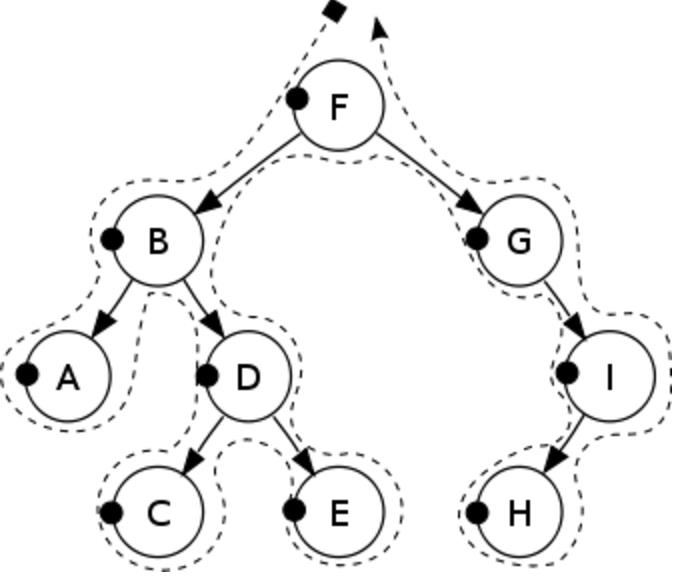
\includegraphics[width=0.3\textwidth]{1.jpg}
\caption{F,B,A,D,C,E,G,I,H}
\end{figure}
\item In-order
\begin{itemize}
\item Traverse the left subtree by recursively calling the in-order function
\clearpage
\item Print the date of the root
\item Traverse the right subtree by recursively calling the in-order function
\end{itemize}
\begin{figure}[h]
\centering
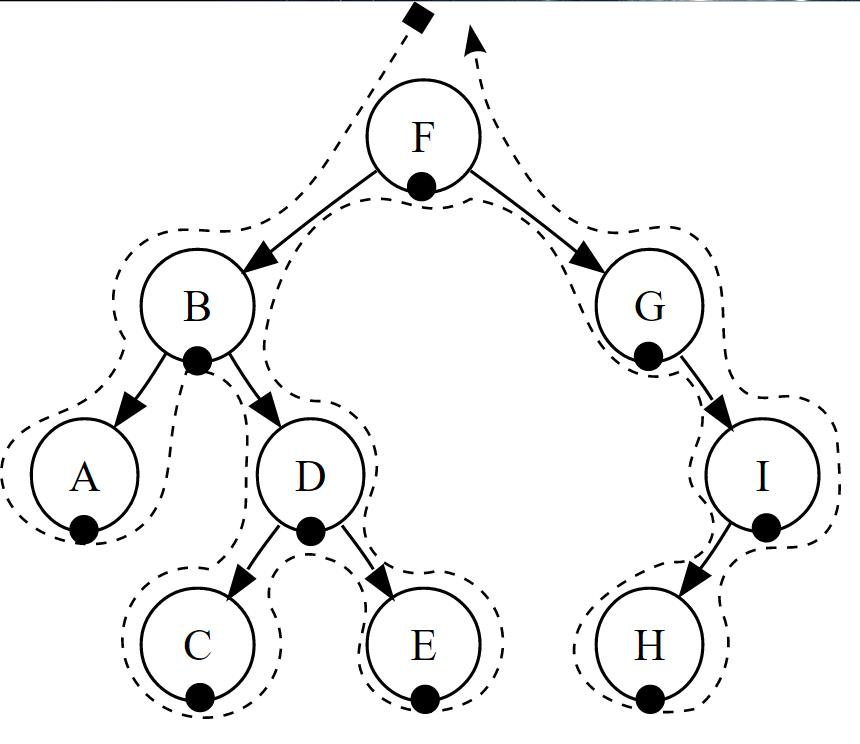
\includegraphics[width=0.3\textwidth]{2.jpg}
\caption{A,B,C,D,E,F,G,H,I}
\end{figure}
\item Post-order
\begin{itemize}
\item Traverse the left subtree by recursively calling the post-order function
\item Traverse the right subtree by recursively calling the post-order function
\item Print the data of the root
\end{itemize}
\begin{figure}[h]
\centering
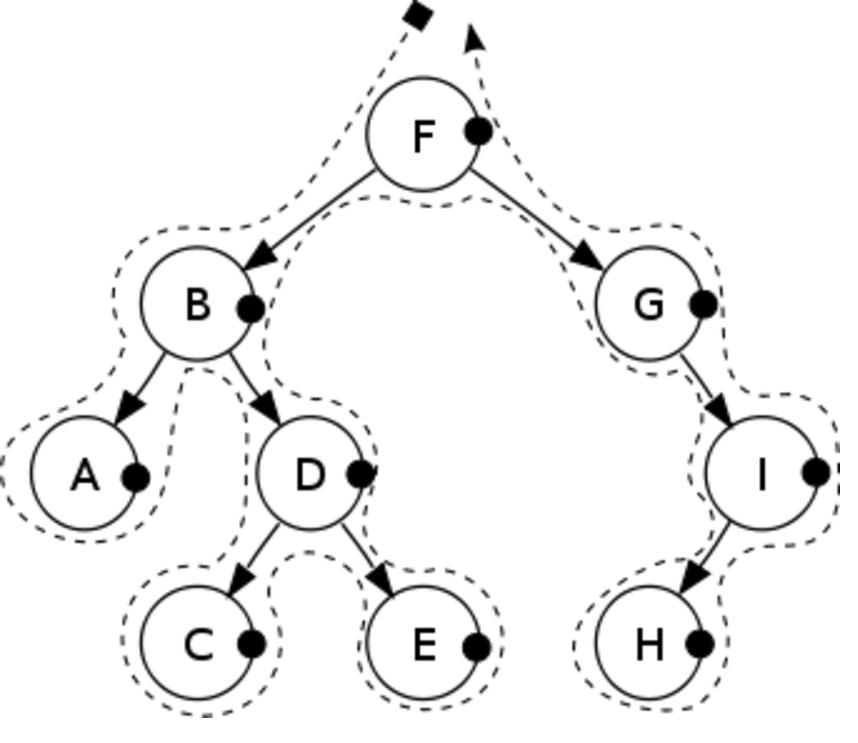
\includegraphics[width=0.3\textwidth]{3.jpg}
\caption{A,C,E,D,B,H,I,G,F}
\end{figure}
\end{itemize}
\subsection{Spanning Trees and Shortest Path}
\begin{definition}[Spanning Tree]
\hfill\\
\normalfont A \textbf{spanning tree} for a graph $G$ is a subgraph of $G$ that contains every vertex of $G$ and is a tree.
\end{definition}
\begin{proposition}[10.7.1]
\hfill\\
\normalfont 
\begin{enumerate}
\item Every connected graph has a spanning tree.
\item Any two spanning trees for a graph have the same number of edges.
\end{enumerate}
\end{proposition}
\begin{definition}[Weighted graph and Minimum Spanning Tree]
\hfill\\
\normalfont A \textbf{weighted graph} is a graph for which each edge has an associated positive real number \textbf{weight}. The sum of the weights of all the edges is the \textbf{total weight} of the graph.\\
A \textbf{mininum spanning tree} for a connected weighted graph is a spanning tree that has the least possible total weight compared to all other spanning trees for the graph.\\
If $G$ is a weighted graph and $e$ is an edge of $G$, then $w(e)$ denotes the weight of $e$ and $w(G)$ denotes the total weight of $G$.
\end{definition}
\begin{algorithm}[Kruskal]
\hfill\\
\normalfont Input: $G$ [a connected weighted graph with $n$ vertices]\\
Algorithm:\\
\begin{enumerate}
\item Initialise $T$ to have all the vertices of $G$ and no edges.
\item Let $E$ be the set of all the edges of $G$, and let $m = 0$.
\item While $(m<n-1)$
\begin{itemize}
\item[3a.] Find an edge $e$ in $E$ of least weight.
\item[3b.] Delete $e$ from $E$.
\item[3c.] If addition of $e$ to the edge set of $T$ does not produce a circuit, then add $e$ to the edge set of $T$ and set $m = m +1$.
\end{itemize}
\item[] End while
\end{enumerate}
\end{algorithm}
\begin{algorithm}[Prim]
\hfill\\
\normalfont Input: $G$ [a connected weighted graph with $n$ vertices]\\
Algorithm:\\
\begin{enumerate}
\item Pick a vertex $v$ of $G$ and let $T$ be the graph with this vertex only.
\item Let $V$ be the set of all vertices of $G$ except $v$.
\item For $i=1$ to $n-1$
\begin{itemize}
\item[3a.] Find an edge $e$ of $G$ such that (1) $e$ connects $T$ to one of the vertices in $V$, and (2) $e$ has the least weight of all eedges connecting $T$ to a vertex in $V$. Let $w$ be the endpoint of $e$ that is in $V$.
\item[3b.] Add $e$ and $w$ to the edge and vertex sets of $T$, and delete $w$ from $V$.
\end{itemize}
\end{enumerate}
Output: $T$ [$T$ is a mininum spanning tree for $G$.]
\end{algorithm}
\begin{algorithm}[Dijkstra]
\hfill\\
\normalfont Input: $G$ [a connected simple graph with positive weight for every edge].$\infty$ [a number greater than the sum of the weights of all the edges in $G$], $w(u,v)$ [the weight of edge $\{u,v\}$], $a$ [the source vertex], $z$ [the destination vertex].\\
Algorithm:\\
\begin{enumerate}
\item[1] Initialise $T$ to be the graph with vertex $a$ and no edges.\\Let $V(T)$ be the set of vertices of $T$, and let $E(T)$ be the set of edges of $T$.
\item[2] Let $L(a)=0$, and for all vertices in $G$ except $a$, let $L(u)=\infty$.\newline[The number $L(x)$ is called the label of $x$.]
\item[3] Initialise $v$ to equal $a$ and $F$ to be $\{a\}$. \newline[The symbol $v$ is used to denote the vertex most recently added to $T$.]\newline
Let $\text{Adj}(x)$ denote the set of vertices adjacent ot vertex $x$.
\item[4] while$(z\notin V(T))$
\begin{itemize}
\item[a.] $F\leftarrow (F-\{v\})\cup\{\text{vertices }\in \text{Adj}(v)\;\text{and}\;\notin V(T)\}$\newline[The set $F$ is the set of fringe vertices.]
\item[b.] For each vertex $u\in\text{Adj}(v)$ and $\notin V(T)$,
\[
\text{if }L(v)+w(v,u)<L(u), then
\]
\[
L(u)\leftarrow L(v)+w(v,u)
\]
\[
D(u)\leftarrow v
\]
\item[c.] Find a vertex $x$ in $F$ with the smallest label.\\ Add vertex $x$ to $V(T)$, and add edge $\{D(x),x\}$ to $E(T)$.\\$v\leftarrow x$
\end{itemize}
\end{enumerate}
Output: $L(z)$ [This is the length of the shortest path from $a$ to $z$]
\end{algorithm}



\clearpage
\section{Appendix 1: Definitions}
This Appendix contains useful definitions from textbook.
\begin{definition}[Even and Odd Numbers]
\hfill\\
\normalfont An integer $n$ is \textbf{even} if, and only if, $n$ equals twice some integer. \\
An integer $n$ is odd, if, and only if, $n$ equals twice some integer plus 1.
\end{definition}

\begin{definition}[Prime Number]
\hfill\\
\normalfont An integer $n$ is \textbf{prime} if, and only if, $n > 1$ and for all positive integers $r$ and $s$, if $n = rs$, then either $r$ or $s$ equals $n$. \\
An integer $n$ is \textbf{composite} if, and only if, $n > 1$ and $n = rs$ for some integers $r$ and $s$ with $1 < r < n$ and $1 < s < n$. 
\end{definition}
\begin{definition}[Rational and Irrational Number]
\hfill\\
\normalfont A real number $r$ is rational if, and only if, it can be expressed as a quotient of twointegers with a nonzero denominator. A real number that is not rational is irrational.\\
More formally, if $r$ is a real number, then
\[
r \text{ is rational}\Leftrightarrow\exists \text{ integers }a\text{ and }b \text{ such that }r=\frac{a}{b}\text{ and } b\neq 0
\]
\end{definition}


\begin{definition}[Root of Polynomial]
\hfill\\
\normalfont A number $c$ is called a root of a polynomial $p(x)$ if, and only if, $p(c) = 0$.

\end{definition}

\begin{definition}[Divisibility]
\hfill\\
\normalfont If $n$ and $d$ are integers and $d\neq 0$ then $n$ is \textbf{divisible} by $d$ if, and only if, $n$ equals $d$ times some integer.\\
Instead of "$n$ is divisible by $d$," we can say that\\
\vspace{-5mm}
\begin{itemize}
\itemsep0em
\item[] $n$ is a multiple of $d$, or
\item[] $d$ is a factor of $n$, or
\item[] $d$ is a divisor of $n$, or
\item[] $d$ divides $n$.
\end{itemize}
The notation $d \mid n$ is read "$d$ divides $n$." Symbolically, if $n$ and $d$ are integers and $d\neq0$:
\[
d \mid n \Leftrightarrow \exists \text{ an integer }k \text{ such that } n = dk.
\]
\end{definition}
\begin{definition}[Standard Factored Form]
\hfill\\
\normalfont Given any integer $n > 1$, the \textbf{standard factored form} of $n$ is an expression of the form
\[n = {p_1}^{e_1} {p_2}^{e_2} \cdots{p_k}^{e_k},\]
where $k$ is a positive integer; $p_1 , p_2 ,\ldots, p_k$ are prime numbers; $e_1 , e_2 ,\ldots, e_k$ are positive integers; and $p_1 < p_2 <\ldots< p_k$.
\end{definition}
\begin{definition}[Decimal Representation]
\hfill\\
\normalfont Given any nonnegative integer $n$, the \textbf{decimal
representation} of $n$ is an expression of the form
\[d_k d_{k-1} \cdots d_2 d_1 d_0,\]
where $k$ is a nonnegative integer; $d_0, d_1, d_2,\ldots, d_k$ (called
the \textbf{decimal digits} of $n$) are integers from 0 to 9 inclusive;
$d_k \neq 0$ unless $n = 0$ and $k = 0$; and
\[n = d_k ·10^k + d_{k-1} ·10^{k-1} +\cdots+ d_2 ·10^2 + d_1 ·10 + d_0.\]
\end{definition}
\begin{definition}[\textit{div} and \textit{mod}]
\hfill\\
\normalfont If $n$ and $d$ are integers and $d > 0$, then
\[ n div d = q \text{and} n mod d = r \Leftrightarrow n = dq + r\]
where $q$ and $r$ are integers and $0 \leq r < d$.
\end{definition}
\begin{definition}[Absolute Value]
\hfill\\
\normalfont For any real number $x$, the \textbf{absolute value} of $x$, denoted $|x|$, is defined as follows:

\begin{equation*}
|x|=\begin{cases}
x &\text{if } x\geq 0\\
-x &\text{if } x<0
\end{cases}
\end{equation*}
\end{definition}
\begin{definition}[Floor]
\hfill\\
\normalfont If $x$ is a real number and $n$ is an integer, then
\[ \floor*{x} = n \Leftrightarrow n \leq x < n + 1.\]
\end{definition}
\begin{definition}[Ceiling]
\hfill\\
\normalfont If $x$ is a real number and $n$ is an integer, then
\[ \ceil*{x} = n \Leftrightarrow n - 1 < x \leq n.\]
\end{definition}
\begin{definition}[Greatest Common Divisor]
\hfill\\
\normalfont Let $a$ and $b$ be integers that are not both zero. The \textbf{greatest common divisor} of $a$
and $b$, denoted $\gcd(a, b)$, is that integer $d$ with the following properties:
\begin{enumerate}
\item $d$ is a common divisor of both $a$ and $b$. In other words,
\[d \mid a \text{ and }d \mid b.\]
\item For all integers $c$, if $c$ is a common divisor of both $a$ and $b$, then $c$ is less than or
equal to $d$. In other words,
\[ \text{for all integers } c,\text{ if }c \mid a \text{ and }c \mid b, \text{ then }c \leq d.\]
\end{enumerate}
\end{definition}
\begin{algorithm}[4.8.2 Euclidean Algorithm]
\hfill\\
$[$Given two integers $A$ and $B$ with $A > B \geq 0$, this algorithm computes $\gcd(A, B)$. It is
based on two facts:
\begin{enumerate}
\item  $\gcd(a, b) = \gcd(b,r)$ if $a, b, q$ and $r$ are integers with $a = b\cdot q + r$ and $0 \leq r < b$.
\item  $\gcd(a, 0) = a.]$
\end{enumerate}
\textbf{Input}: $A$, $B$ [integers with $A > B \geq 0$]
\textbf{Algorithm Body}:
\begin{itemize}
\item[] $a := A, b := B,r := B$
\item[] [If $b \neq 0$, compute $a \mod b$, the remainder of the integer division of $a$ by $b$, and set $r$ equal to this value. Then repeat the process using $b$ in place of $a$ and $r$ in place of $b$.]
\item[] \textbf{while} ($b\neq 0$)
\item[] \hspace{5em}$r := a \mod b$
\item[] [The value of $a \mod b$ can be obtained by calling the division algorithm.]
\item[] \hspace{5em}$a := b$
\item[] \hspace{5em}$b := r$
\item[] \textbf{end while}
\item[] [After execution of the \textbf{while} loop, $\gcd(A, B) = a$.]
\item[] $\gcd$ := a
\end{itemize}
\textbf{Output}: $\gcd$ [a positive integer]
\end{algorithm}
\begin{definition}[Modulo]
\hfill\\
\[m \equiv n \pmod{ d} \Leftrightarrow d \mid (m - n)\]
\end{definition}
\begin{definition}[Linear Combination of Integer]
\hfill\\
\normalfont An integer $d$ is said to be a \textbf{linear combination of integers} $a$ and $b$ if, and only if,
there exist integers $s$ and $t$ such that $as + bt = d$.
\end{definition}
\begin{definition}[Coprime]
\hfill\\
\normalfont Integers $a$ and $b$ are \textbf{relatively prime} if, and only if, $\gcd(a, b) = 1$. Integers $a_1, a_2,
a_3,\ldots, a_n$ are \textbf{pairwise relatively prime} if, and only if, $\gcd(a_i, a_j) = 1$ for all integers
$i$ and $j$ with $1 \leq i, j \leq n$, and $i \neq j$.
\end{definition}
\begin{definition}[Inverse Relation]
\hfill\\
\normalfont Let $\mathcal{R}$ be a relation from $A$ to $B$. Define the inverse relation $\mathcal{R}^{-1}$ fom $B$ to $A$ as follows:
\[
\mathcal{R}^{-1}=\{(y,x)\in B\times A\mid(x,y)\in \mathcal{R}\}
\]
\end{definition}
\clearpage
\section{Appendix 2: Theorems}
\begin{theorem}[4.1.1]
\hfill\\
\normalfont The sum of any two even integers is even.
\end{theorem}
\begin{theorem}[4.2.1]
\hfill\\
\normalfont Every integer is a rational number.
\end{theorem}
\begin{theorem}[4.2.2]
\hfill\\
\normalfont The sum of any two rational numbers is rational.
\end{theorem}
\begin{theorem}[4.3.1]
\hfill\\
\normalfont For all integers $a$ and $b$, if $a$ and $b$ are positive and $a$ divides $b$, then $a \leq b$.
\end{theorem}
\begin{theorem}[4.3.2]
\hfill\\
\normalfont The only divisors of 1 are 1 and -1.
\end{theorem}
\begin{theorem}[4.3.3]
\hfill\\
\normalfont For all integers $a, b$, and $c$, if $a$ divides $b$ and $b$ divides $c$, then $a$ divides $c$.
\end{theorem}
\begin{theorem}[4.3.4]
\hfill\\
\normalfont Any integer $n > 1$ is divisible by a prime number.
\end{theorem}
\begin{theorem}[4.3.5]
\hfill\\
\normalfont Given any integer $n > 1$, there exist a positive integer $k$, distinct prime numbers $p_1 , p_2 ,\ldots, p_k$ , and positive integers $e_1 , e_2 ,\ldots, e_k$ such that
\[n = {p_1}^{e_1} {p_2}^{e_2} \cdots{p_k}^{e_k},\]
and any other expression for $n$ as a product of prime numbers is identical to this except, perhaps, for the order in which the factors are written.
\end{theorem}
\begin{theorem}[4.4.1]
\hfill\\
\normalfont Given any integer $n$ and positive integer $d$, there exist unique integers $q$ and $r$ such
that
\[n=dq+r \text{ and } 0\leq r<d\]
\end{theorem}
\begin{theorem}[4.4.2]
\hfill\\
\normalfont Any two consecutive integers have opposite parity.
\end{theorem}
\begin{theorem}[4.4.3]
\hfill\\
\normalfont The square of any odd integer has the form $8m + 1$ for some integer $m$.
\end{theorem}
\begin{lemma}[4.4.4]
\hfill\\
\normalfont For all real numbers $r$, $-|r| \leq r \leq |r|$.
\end{lemma}
\begin{lemma}[4.4.5]
\hfill\\
\normalfont For all real numbers $r$, $| - r|=|r|$.
\end{lemma}
\begin{theorem}[4.4.6]
\hfill\\
\normalfont For all real numbers $x$ and $y$, $|x + y|\leq|x|+|y|$. 
\clearpage
\end{theorem}
\begin{theorem}[4.5.1]
\hfill\\
\normalfont For all real numbers $x$ and all integers $m$, $\floor*{x+m}=\floor*{x}+ m$.
\end{theorem}
\begin{theorem}[4.5.2]
\hfill\\
\normalfont For any integer $n$,
\begin{equation*}
\floor{\frac{x}{2}}=\begin{cases}
\frac{n}{2}&\text{if }n \text{ is even}\\
\frac{n-1}{2} &\text{if } n \text{ is odd}
\end{cases}
\end{equation*}
\end{theorem}
\begin{theorem}[4.5.3]
\hfill\\
\normalfont If $n$ is any integer and $d$ is a positive integer, and if $q = \floor*{n/d}$ and $r = n - d\floor*{n/d}$, then
\[n = dq + r \text{ and } 0 \leq r < d.\]
\end{theorem}
\begin{theorem}[4.6.1]
\hfill\\
\normalfont There is no greatesst integer.
\end{theorem}
\begin{theorem}[4.6.2]
\hfill\\
\normalfont There is no integer that is both even and odd.
\end{theorem}
\begin{theorem}[4.6.3]
\hfill\\
\normalfont The sum of any rational number and any irrational number is irrational.
\end{theorem}
\begin{proposition}[4.6.4]
\hfill\\
\normalfont For all integers $n$, if $n^2$ is even then $n$ is even.
\end{proposition}
\begin{theorem}[4.7.1]
\hfill\\
\normalfont $\sqrt{2}$ is irrational.
\end{theorem}
\begin{proposition}[4.7.3]
\hfill\\
\normalfont For any integer $a$ and any prime number $p$, if $p \mid a$ then $p \nmid (a + 1)$.
\end{proposition}
\begin{proposition}[4.7.4]
\hfill\\
\normalfont The set of prime numbers is infinite.
\end{proposition}
\begin{lemma}[4.8.1]
\hfill\\
\normalfont If $r$ is a positive integer, then $\gcd(r, 0) = r$.
\end{lemma}
\begin{lemma}[4.8.2]
\hfill\\
\normalfont If $a$ and $b$ are any integers not both zero, and if $q$ and $r$ are any integers such that
$a = bq + r$, then $\gcd(a, b) = \gcd(b,r)$.
\end{lemma}
\begin{theorem}[5.2.2]
\hfill\\
\normalfont For all integers $n \geq 1$,
\[1 + 2 +\cdots+ n = \frac{n(n + 1)}{2}.\]
\end{theorem}
\begin{theorem}[5.2.3]
\hfill\\
\normalfont For any real number $r$ except 1, and any integer $n \geq 0$,
\[
\Sigma^{n}_{i=0}r^i = \frac{r^{n+1}-1}{r-1}
\]
\end{theorem}
\begin{proposition}[5.3.1]
\hfill\\
\normalfont For all integers $n \geq 0$, $2^{2n} - 1$ is divisible by 3.
\end{proposition}
\begin{proposition}[5.3.2]
\hfill\\
\normalfont For all integers $n ≥\geq 3$, $2n + 1 < 2^n$.
\end{proposition}
\begin{theorem}[5.4.1]
\hfill\\
\normalfont Given any positive integer $n$, $n$ has a unique representation in the form
\[n = c_r \cdot 2^r + c_{r-1} \cdot 2^{r-1} +\cdots+ c_2 ·2^2 + c_1 \cdot 2 + c_0,\]
where $r$ is a nonnegative integer, $c_r = 1$, and $c_j = 1 \text{ or }0 \text{ for all }j = 0, 1, 2,\ldots,r - 1$.
\end{theorem}
\begin{theorem}[Well Ordering Principle for the Integers]
\hfill\\
\normalfont Let $S$ be a set of integers containing one or more integers all of which are greater
than some fixed integer. Then $S$ has a least element.
\end{theorem}
\begin{theorem}[8.4.1]
\hfill\\
\normalfont Let $a, b$ and $n$ be any integers and suppose $n > 1$. The following statements are all
equivalent:
\begin{enumerate}
\item $n \mid(a - b)$
\item $a \equiv b \pmod{n}$
\item $a = b + kn$ for some integer $k$
\item $a$ and $b$ have the same (nonnegative) remainder when divided by $n$
\item $a \pmod{n}= b\pmod{n}$
\end{enumerate}
\end{theorem}
\begin{theorem}[8.4.3]
\hfill\\
\normalfont Let $a, b, c, d$ and $n$ be integers with $n > 1$, and suppose
\[a \equiv c \pmod{n} \text{ and } b \equiv d \pmod{n}\]
Then
\begin{enumerate}
\item $(a + b) \equiv (c + d) \pmod{n}$
\item $(a - b) \equiv (c - d) \pmod{n}$
\item $ab \equiv cd \pmod{n}$
\item $a^m \equiv c^m \pmod{n}$ for all integers $m$.
\end{enumerate}
\end{theorem}
\begin{corollary}[8.4.4]
\hfill\\
\normalfont Let $a, b$ and $n$ be integers with $n > 1$. Then
\[ab \equiv [(a \bmod n)(b \bmod n)]\pmod{n},\]
or, equivalently,
\[ab \bmod n = [(a \bmod n)(b \bmod n)] \bmod n.\]
In particular, if $m$ is a positive integer, then
\[a^m \equiv [(a \bmod n)^m]\pmod{n}.\]
\end{corollary}
\begin{theorem}[8.4.5]
\hfill\\
\normalfont For all integers $a$ and $b$, not both zero, if $d = \gcd(a, b)$, then there exist integers $s$
and $t$ such that $as + bt = d$.
\end{theorem}
\begin{corollary}[8.4.6]
\hfill\\
\normalfont If $a$ and $b$ are relatively prime integers, then there exist integers $s$ and $t$ such that
$as + bt = 1$.
\end{corollary}
\begin{corollary}[8.4.7]
\hfill\\
\normalfont For all integers $a$ and $n$, if $\gcd(a, n) = 1$, then there exists an integer $s$ such that
$as \equiv 1 \pmod{n}$. The integer $s$ is called the \textbf{inverse of a modulo n}.
\end{corollary}
\begin{lemma}[8.4.8]
\hfill\\
\normalfont For all integers $a, b$ and $c$, if $\gcd(a, c) = 1$ and $a \mid bc$, then $a \mid b$.
\end{lemma}
\begin{theorem}[8.4.9]
\hfill\\
\normalfont For all integers $a, b, c$ and $n$ with $n>1$, if $\gcd(c, n) = 1$ and $ac \equiv bc \pmod{n}$, then
$a \equiv b \pmod{n}$.
\end{theorem}
\begin{theorem}[8.4.10]
\hfill\\
\normalfont If $p$ is any prime number and $a$ is any integer such that $p \nmid a$, then $a^{p-1} \equiv 1 \pmod{p}$.
\end{theorem}
\begin{theorem}[7.1.1]
\hfill\\
\normalfont If $f:X\to Y$ and $g:X\to Y$ are functions, then $f=g$ if, and only if, $f(x)=g(x)$ for all $x\in X$.
\end{theorem}
\begin{theorem}[7.2.3]
\hfill\\
\normalfont If $X$ and $Y$ are sets and $f:X\to Y$ is one-to-one and onto, then $f^{-1}:Y\to X$ is also \textbf{one-to-one} and \textbf{onto}.
\end{theorem}
\begin{theorem}[7.3.1]
\hfill\\
\normalfont If $f$ is a function from a set $X$ to a set $Y$, and $I_X$ is the identity function on $X$, and $I_Y$ is the identity function on $Y$, then
\[
f\circ I_X = f, I_Y\circ f=f
\]
\end{theorem}
\begin{theorem}[7.3.3]
\hfill\\
\normalfont If $f:X\to Y$ and $g:Y\to Z$ are both one-to-one functions, then $g\circ f$ is one-to-one.
\end{theorem}
\begin{theorem}[7.3.4]
\hfill\\
\normalfont If $f:X\to Y$ and $g:Y\to Z$ are both onto functions, then $g\circ f$ is onto.
\end{theorem}
\begin{theorem}[9.2.2]
\hfill\\
\normalfont For any integer $n$ with $n\geq 1$, the number of permutations of a set with $n$ elements is $n!$.
\end{theorem}




\clearpage
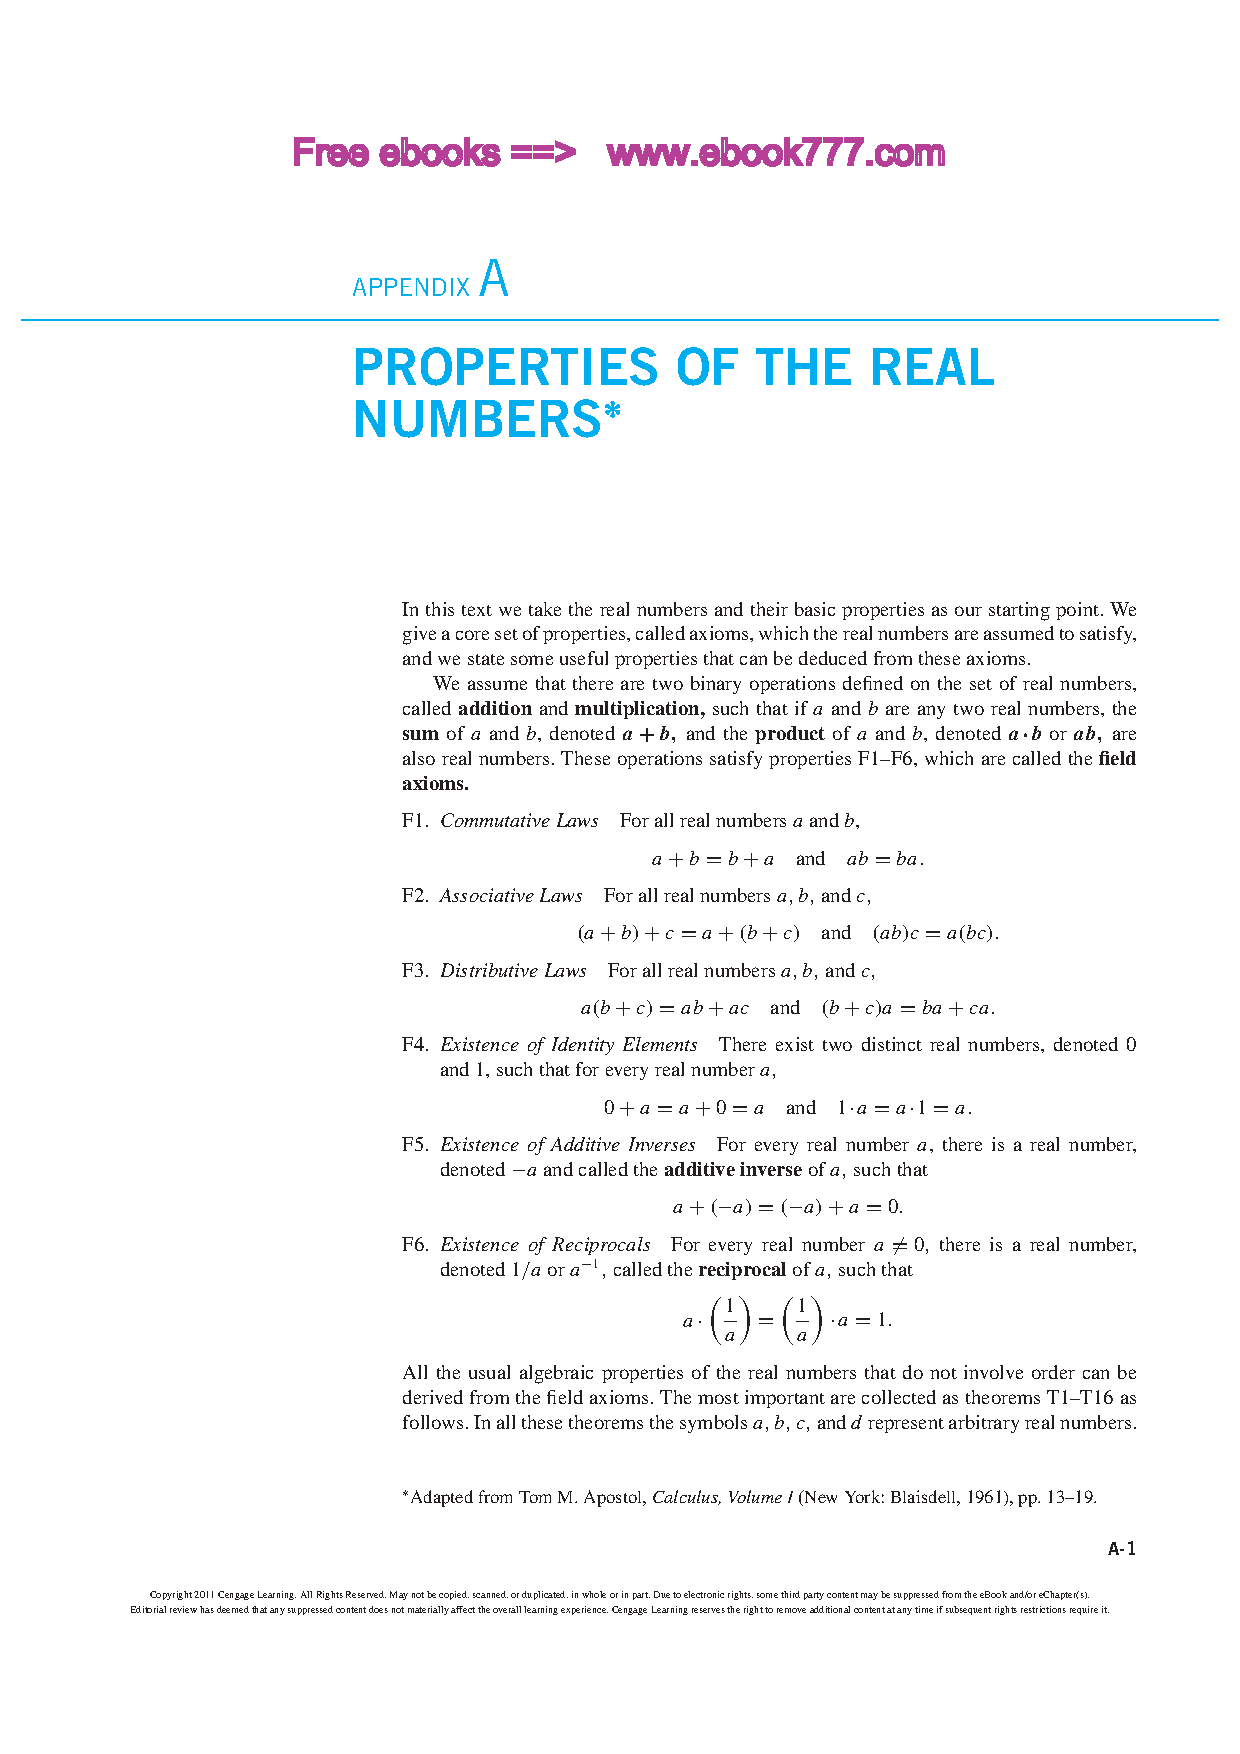
\includepdf[pages={1-3}]{appendix1.pdf}
\clearpage

\end{document}

